\documentclass[10pt]{article}
\oddsidemargin = 0.2in
\topmargin = -0.5in
\textwidth 6in
\textheight 8.5in

\usepackage{graphicx,bm,amssymb,amsmath,amsthm} % Figures and maths
\usepackage{xcolor}
\usepackage[colorlinks]{hyperref} % Hyperlinks
\usepackage[capitalise, nameinlink]{cleveref} % Better referencing
\crefname{equation}{}{} % Cref shows eqs as (n) rather than Eq. (n)
\usepackage{array}
\usepackage{showlabels} % Shows eq, fig, etc labels
\usepackage{siunitx} % SI units
\usepackage[caption=false]{subfig} % For subfloats
\usepackage{bold-extra} % bold for texttt
\usepackage{bm} % bold for maths 
\usepackage{tabularx} % for nice tables
\usepackage[export]{adjustbox} % for adjusting the alignment of subfigures
% Tikz figures
\usepackage{tikz}
\usepackage[most]{tcolorbox}
\usetikzlibrary{positioning}
\usepackage{comment}                % to comment out big blocks


% SI unit definitions
\DeclareSIUnit\parsec{pc}

% -------------------------------------- macros --------------------------
% general ...
\newcommand{\bi}{\begin{itemize}}
\newcommand{\ei}{\end{itemize}}
\newcommand{\ben}{\begin{enumerate}}
\newcommand{\een}{\end{enumerate}}
\newcommand{\be}{\begin{equation}}
\newcommand{\ee}{\end{equation}}
\newcommand{\bea}{\begin{eqnarray}} 
\newcommand{\eea}{\end{eqnarray}}
\newcommand{\ba}{\begin{align}} 
\newcommand{\ea}{\end{align}}
\newcommand{\bse}{\begin{subequations}} 
\newcommand{\ese}{\end{subequations}}
\newcommand{\bc}{\begin{center}}
\newcommand{\ec}{\end{center}}
\newcommand{\bfi}{\begin{figure}}
\newcommand{\efi}{\end{figure}}
\newcommand{\ca}[2]{\caption{#1 \label{#2}}}
\newcommand{\ig}[2]{\includegraphics[#1]{#2}}
\newcommand{\bmp}[1]{\begin{minipage}{#1}}
\newcommand{\emp}{\end{minipage}}
\newcommand{\pig}[2]{\bmp{#1}\includegraphics[width=#1]{#2}\emp} % mp-fig, nogap
\newcommand{\bp}{\begin{proof}}
\newcommand{\ep}{\end{proof}}
\newcommand{\ie}{{\it i.e.\ }}
\newcommand{\eg}{{\it e.g.\ }}
\newcommand{\etal}{{\it et al.\ }}
\newcommand{\etc}{{\it etc.\ }}
\newcommand{\pd}[2]{\frac{\partial #1}{\partial #2}}
\newcommand{\pdc}[3]{\left. \frac{\partial #1}{\partial #2}\right|_{#3}}
\newcommand{\infint}{\int_{-\infty}^{\infty} \!\!}      % infinite integral
\newcommand{\tbox}[1]{{\mbox{\tiny #1}}}
\newcommand{\mbf}[1]{{\mathbf #1}}
\newcommand{\half}{\mbox{\small $\frac{1}{2}$}}
\newcommand{\C}{\mathbb{C}}
\newcommand{\N}{\mathbb{N}}
\newcommand{\R}{\mathbb{R}}
\newcommand{\Z}{\mathbb{Z}}
\newcommand{\RR}{\mathbb{R}^2}
\renewcommand{\d}{\mathrm{d}} % Upright differential
\newcommand{\ve}[4]{\left[\begin{array}{r}#1\\#2\\#3\\#4\end{array}\right]}  % 4-col-vec
\newcommand{\vt}[2]{\left[\begin{array}{r}#1\\#2\end{array}\right]} % 2-col-vec
\newcommand{\bigO}{{\mathcal O}}
\newcommand{\qqquad}{\qquad\qquad}
\newcommand{\qqqquad}{\qqquad\qqquad}
\newcommand{\eps}{\epsilon}
\newcommand{\veps}{\varepsilon}
\DeclareMathOperator{\Span}{Span}
\DeclareMathOperator{\im}{Im}
\DeclareMathOperator{\re}{Re}
\DeclareMathOperator{\vol}{vol}
\newtheorem{thm}{Theorem}
\newtheorem{cnj}[thm]{Conjecture}
\newtheorem{lem}[thm]{Lemma}
\newtheorem{cor}[thm]{Corollary}
\newtheorem{pro}[thm]{Proposition}
\newtheorem{rmk}[thm]{Remark}
\newtheorem{defn}[thm]{Definition}
% this work...
\newcommand{\om}{\omega}
\newcommand{\g}{\gamma}
\newcommand{\te}{\tilde\eta}
\crefalias{prop}{Proposition}
% Review
\newcommand{\AB}[1]{{\color{orange}#1}}
\newcommand{\Fruzsi}[1]{{\color{blue}#1}}

\begin{document}

\title{An adaptive spectral method for oscillatory second-order linear ODEs with frequency-independent cost }

\author{Fruzsina J.\ Agocs and Alex H.\ Barnett}
\maketitle

\begin{abstract}

% Main points to communicate:
% * Presenting a method for second order linear ODEs whose solution may be highly oscillatory
% * Spectral, adaptive -- can deal with oscillatory or slowly varying solutions
% * Based on constructing a nonoscillatory phase function (which obeys the Riccati equation)
% via defect correction which yields an asymptotic series,
% geometric/exponential convergece in residual for first few iters
% * Chebyshev spectral method is alternative solver
% * We demonstrate performance with numerical examples, results

% 168 words!

We introduce an efficient numerical method for second order linear ODEs whose
solution may vary between highly oscillatory and slowly changing over the solution interval.
%
In oscillatory regions the solution is generated via a nonoscillatory phase
function that obeys the nonlinear Riccati equation.
%
We propose a
defect-correction iteration that gives an asymptotic series for such a phase
function; this is numerically approximated on a Chebyshev grid with a small number of nodes.
%
For analytic coefficients we prove that each iteration, up to a certain
maximum number,
reduces the residual by a factor of order of the local frequency. 
%
The algorithm adapts both the step size and the choice of method,
switching to a conventional spectral collocation method
away from oscillatory regions.
%method based on an adaptively varied number of Chebyshev nodes.
% FA: The number of Cheby nodes is actually adaptive --> change back?
%
In numerical experiments we find that our proposal outperforms other state-of-the-art
oscillatory solvers, most significantly at low-to-intermediate
frequencies and at low tolerances, where it may use up to $10^6$
times fewer function evaluations.  Even in high frequency regimes, our
implementation is
% AB: we have to be careful about claims re the method vs the implementation
on average $10$ times faster than other specialised solvers.
\end{abstract}

\section{Introduction}\label{introduction}

The efficient numerical solution of highly oscillatory ordinary differential
equations (ODEs) has long been a challenge.
A wide range of specialised methods exists for dealing with ODEs
with various structures;
see \cite{petzold1997,engquist2009} for thorough reviews.
In this work we handle a commonly occurring
form, the variable-coefficient, linear, second
order ODE with
% \Fruzsi{analytic} % numerical method could handle merely smooth.
smooth coefficients.
This includes simple % you didn't mean "single", right?
harmonic oscillators with time-dependent coefficients,
which arise in many computational physics problems.
% note I cut "simple-looking". not needed
One application in which an extremely fast numerical solution is needed
is Bayesian parameter estimation in cosmology.
Specifically, each spatial Fourier mode of the density pertubations
obeys such an ODE in time,
with solutions that may switch repeatedly between smooth and
highly oscillatory characters \cite{agocs2020dense}.
Of order $10^3$ modes are needed, and this must be repeated for
up to $10^6$ trial parameter choices; thus the ODE solver
may be called a billion times, and an efficient frequency-independent
solver is crucial.
Besides inflationary cosmology \cite{Hergt2022,martin2003,winitzki2005}, this class of ODE appears in
Hamiltonian dynamics \cite{Pritula2018,fiore2022}, particle accelerators and plasma physics
\cite{courant1958,davidson2001,hazeltine2003,lewis1968}, electric circuits
\cite{likharev2022}, satellite systems \cite{saxena2020}, acoustics and gravity waves \cite{filippi1998,einaudi1970}, and quantum mechanics \cite{griffiths2018,adhikari1988,arnold2011wkb,cea1982}.
In many of these fields our proposed method could supply a robust and efficient
numerical replacement for
uncontrolled asymptotic approximations.
%which at high order can become cumbersome to apply.
%  https://www.math.leidenuniv.nl/~vivi/stud_sem2011/BosleyKevorkian92.pdf  latex fail -> coupled oscillators

% Define the problem completely before you start getting into details about complex omega:
The ODE under study has the form
\be
u''(t) + 2\g(t) u'(t) + \om^2(t)u(t) = 0, \quad t \in (t_0,t_1) \subset \R,
\label{ode}
\ee
where $\g$ is a given smooth (by which we mean $C^\infty$) damping function,
and $\om$ is a given smooth, but possibly very large, real-valued
local frequency function\footnote{If coefficients are merely piecewise smooth, a solution may simply be patched together at the breakpoints, thus we do not discuss this situation further.}.
We solve the initial value problem (IVP)
\begin{align} % \ba, \ea doesn't work here, LaTeX complains
    u(t_0) &= u_0, \label{ic0} \\
    u'(t_0) &= u'_0, \label{ic1}
\end{align}
although we note that the methods that we present could easily be applied to
two-point boundary value problems.
%Here the local frequency function $\om(t)$ is purely real or purely imaginary.
% AB: so is om(t) complex or real?
% FA: technically it could be complex. The issue is when we try to use a spectral method over complex coefficients.
% AB: Hmmm, really, why does that go wrong?
% FA: I would expect it to pick up the exponentially growing mode -- but not so sure now.
The restriction to real $\om$ is not crucial,
but avoids complications with exponentially large dynamic ranges
(e.g., deeply evanescent regions)
that we leave for future study.
%For now, we only consider the case when $\om$ is purely real, but note that our
%asymptotic approximation for the Riccati phase function described in
%\cref{phasefun} is applicable to complex $\om$.
% consider cut or footnote. Notice it forced you to explain stuff we're going to explain shortly anyway, so it's confusing.
%
%Care needs to be taken in
%regions of $\Im(\om) \neq 0$ if any other method is used, however, since due to
%roundoff error some of the exponentially growing solution will inevitably be
%picked up and will dominate over the evanescent solution\footnote{In quantum
%mechanical applications where having a purely imaginary $\om$ is ubiquitous, a
%workaround is to integrate the ODE from outside the edges of the potential well
%towards the inside.}. We defer allowing for complex $\om$ to future work.

In regions where $\om \gg 1$,
the solution $u$ is oscillatory:
loosely speaking,
it has local approximate form $a e^{i\om_0t} + b e^{-i\om_0t}$, where $\om_0$
is a local value of $\om(t)$.
Conventional ODE integrators then require discretization with several
grid points per local period $2\pi/\om_0$, forcing the overall
cost to be $\bigO(\om_0)$, which can be prohibitively slow.
This has led to the development of solvers
that exploit new representations or asymptotic expansions of the solution, allowing many periods between discretization nodes.
% AB: note the following waypoint to the reader re the big section about to happen:
We now review such prior work,
while noting that, to our knowledge, our proposal is the first
tackle the problem adaptively with spectral accuracy
when the solution has both highly oscillatory and smooth regimes.

% WKB
The most common asymptotic expansion
is the Wentzel--Kramers--Brillouin (WKB), a
perturbation method applied to linear differential equations that contain a
small parameter
%$\varepsilon$  <- this is never used later so no symbol is needed
in the highest derivative
\cite{benderorszag,logan}.
This approximation arose in quantum mechanics where it is still widely
applied for approximate analytic solutions of the Schr\"{o}dinger equation.
Writing $\om(t) = \om_0\Omega(t)$,
where $\Omega(t)$ is of unit size, and the asymptotic parameter is
$\om_0 \gg 1$,    % AB: note how I cut down here
% AB: oops not \ll
% AB: note you don't set gam=0 until later, so I fixed that
\cref{ode} becomes
\be\label{odewkb}
u'' + 2\gamma u' + \om_0^2 \Omega^2 u = 0.
\ee
Substituting $u(t) = e^{\om_0 z(t)}$ and defining $z'(t) = x(t)$
% AB note how I cue the reader these are functions of t
gives the Riccati equation (a nonlinear 1st-order ODE) for $x$, 
\be\label{riccwkb}
% AB please debug if om_0^2 here ???
% FA: No bugs here, note the exponent in the substitution contains om_0, which kills one factor of om_0.
x' + 2\gamma x + \om_0 x^2 + \om_0 \Omega^2 = 0.
\ee
Making a regular perturbation expansion in $1/\om_0$,
\be\label{wkbexpansion}
x(t) = \sum_{j=0}^{N} \om_0^{-j} x_j(t),
% AB note how I put consts before funcs (traditional) and cue the reader re funcs of t, not merely numbers.
\ee
and matching powers of $\om_0$ in \cref{odewkb} gives the recursion relation
for the functions $x_j(t)$
(where for simplicity we give only the $\gamma \equiv 0$ case),
\begin{equation}\label{wkbrecur}
  x_0 = \pm i\Omega, \quad x_j = -\frac{1}{2x_0}\left( x'_{j-1} + \sum_{k = 1}^{j-1}x_k x_{j-k} \right), \quad \text{for } j = 1, 2, \ldots.
\end{equation}
Although originally an analytic tool,
WKB has recently been exploited in numerical solvers.
These algorithms achieve
$\bigO(1)$ (\ie $\om_0$-independent) runtime in regions where the asymptotic
series is a sufficiently good approximation.
WKB forms the basis of the method described in
\cite{agocs2020efficient,agocs2020dense}, and associated open-source software
package \texttt{oscode} \cite{agocs2020joss}. This uses the expansion
\cref{wkbexpansion} up to and including $x_3$ within a time-step,
or, if this is not accurate enough, switches to a 4,5th
order Runge--Kutta pair.
% AB: note "isn't" is too casual. Also, keeping concise.
In \cite{arnold2011wkb,korner2022wkb} the related
``WKB marching method'' uses the same
expansion truncated after $x_2$ to transform \cref{odewkb} into a smoother
problem in the highly oscillatory regions,
otherwise again switching to a 4,5th order Runge--Kutta method.
%
In terms of the stepsize $h$, neither method is formally high-order.
\texttt{oscode} has
$\bigO(h)$ global error, although
its prefactor is small when $\om_0$ is large.
%error when $h \ll 1$, although in regions of high-frequency oscillations, $h$
%tends to be very large in comparison to the solution's timescale.
The
WKB-marching method's oscillatory solver improves on this and has $\bigO(h^2)$ global error, resulting in better performance at lower tolerances.
% AB I feel a clearer way to say would be error is O(h^2 / om^3) or something... for each solver.
% FA: OK. For WKB marching, they have the global error $\leq C(h^{g}\om + h^2/\om^3)$.
% The $g$ is the order of a quadrature routine involved, which
% can be chosen. They say that even though the first term scales badly with
% $\om$, it sometimes goes away due to the relevant integral having an analytic
% solution. For Bremer, the global error of the method is a little unclear:
% there is an approximate solution to an approximation of Kummer's equation,
% and each of these have an error, but I don't know how they combine. For
% oscode, we never investigated the error in terms of $\om$, so I only know
% it's globally $\bigO(h)$. For our method, I'm not sure how the Riccati
% method's error scales with $h$ -- the error depends on bounds on $\om$ over
% [t, t+h]. I think the same goes for oscode. Can we discuss in a call/email?

Yet, as a consequence of low $h$ order and fixed asymptotic order,
a small requested tolerance in either method forces
$h \lesssim 1/\om_0$, removing the efficiency advantage over conventional timesteppers.
%which in turn causes them to switch over to their respective Runge--Kutta solvers 
%even if the solution is oscillatory.
They are therefore only efficient if no more than about 6 digits of accuracy
are required, and can suffer at low-to-intermediate frequencies where more asymptotic terms would be required.
The present method, on the other hand, is both spectrally accurate and 
adaptive in the number of terms in its asymptotic expansion.

%The local error of our proposed
%method's Riccati steps depends on the stepsize $h$ in two
%ways: first, the asymptotic expansion's validity is determined by the magnitude
%and rate-of-change of $\om$ and $\g$ over the course of the step (formalised in
%\cref{errorana}); and second, the iterates $x_i$ are computed via numerical
%differentiation on a Chebyshev grid with an adaptive number of nodes, which has
%$\bigO(h^{n+1-k})$ accuracy if the number of iterates included is $k$. In this
%sense, both of the methods making up our solver are arbitrarily high order.
%\AB{Valiant, but I think too much detail here. Just say we are spectral. Move detail to discussion}

% QLM
%Instead of finding an approximation via a regular perturbative expansion, the
The ``quasilinearisation method''
% note M stands for method, so approach was bit confusing
(QLM) \cite{bellman1970} instead successively approximates
a solution of the Riccati equation \cref{riccwkb}
by a functional Newton iteration.
The resulting differential equation recurrence (here stated for $\gamma\equiv 0$),
\be
x_0 = \pm i\om, \quad
x_j' - x_{j-1}^2 + 2x_j x_{j-1} + \om^2 = 0, \quad \text{for } j = 1, 2, \ldots
\label{qlmode}
\ee
turns out to yield a solution equivalent to a WKB expansion with $2^j$ terms.
This recurrence is either solved symbolically \cite{mandelzweig2004,krivec2006}
or numerically \cite{krivec2008,krivec2014}. The former
requires increasing amounts of algebra with iteration number, so can
become cumbersome. Integrating each ODE in \cref{qlmode} numerically does not prove to be a better strategy since each such ODE is itself oscillatory.

% Bremer
% Accuracy?
% arbitrarily high order
Recently Bremer \cite{bremer2018}, following \cite{heitman2015,bremer2016},
has proposed an efficient
method for solving \cref{ode}, in the special case $\g = 0$,
over a domain in which the solution is highly oscillatory.
%\AB{Is this distinct from the WKB methods just described?
%  Ie, don't they also run in $\bigO(1)$ time?
%  In which case I suggest we state that above, and not make it a new property here.
%  To me the Bremer innovation is high-order approximation of phase func
%  on intervals,
%  plus convergence, plus code.}
The method aims to find a global nonoscillatory phase function $\alpha(t)$
satisfying Kummer's equation,
\be
\frac{3}{4} \left(\frac{\alpha''}{\alpha'}\right)^2 - \frac{1}{2}\frac{\alpha'''}{\alpha'} - (\alpha')^2 +
\om(t)^2 = 0,
\label{kummer}
\ee
a nonlinear and generally oscillatory ODE, and will therefore be referred to as the Kummer's phase function method hereafter.
% AB: our method is also a PF meth, so let's not do that ^.
%
One then reconstructs solutions
via $u(t) = \sin(\alpha(t) + c)/\sqrt{\alpha'(t)}$.
% AB: note the reader benefits from seeing how it relates to u
%
%The nonoscillatory phase function $\alpha$ can be used to compute an approximation
%of the solution of \cref{riccwkb} accurate to within
%$\bigO((\mu\om_0)^{-1}\exp(-\mu\om_0))$ as $\om_0 \to \infty$, where $\mu$ is a constant that depends on $\Omega(t)$ but not $\om_0$.
% AB ***: I found that confusing - I thought Bremer did not use Riccati form?
% FA: My bad, instead of riccwkb, it should have pointed to the original ODE.
% I decided to cut error detail
%
%The proposed algorithm itself generates $\tilde{\alpha}$, an approximation
%of $\alpha$, such that the so-called logarithm form of Kummer's
%equation is satisfied to within $\bigO(-\tfrac{1}{2}\mu\om_0)$.
% AB: *** somethign wrong there _^  what do you mean?  Also too much detail, so I cut.
% FA: I mean that the error in the prev paragraph would be the global error if
% $\alpha$ were computed exactly. But it is not. Bremer says that "we describe
% a methdod for constructing a solution of the logarithm form of Kummer’s
% equation whose difference from the nonoscillatory solution of (<approximate
% form of log Kummer's eq>) is on the order of $\exp{-1/2\mu\om_0}$".  
The generated phase functions are nonoscillatory in the sense that they can be
accurately approximated on intervals of fixed size
using polynomials of degree independent of $\om_0$.
%(\eg via Chebyshev polynomials)
%with $\bigO(1)$ terms,
The results of \cite{heitman2015,bremer2016}
prove the existence of such nonoscillatory phase functions when
$\Omega(t)$ is
nonoscillatory in the sense that $\log \Omega$ is smooth and its Fourier transform rapidly decaying.
% *** AB check do you really mean smooth? since it has to be smooth in Fourier
% due to compactness of interval. Please check.
% FA: I checked and corrected: log \Omega has to be smooth and its Fourier transform rapidly decaying.
Finding initial conditions on the phase function leading to
a nonoscillatory solution is, however, challenging.
Bremer proposed a ``windowing'' method to numerically find such a global phase function on the interval $(t_0,t_1)$,
% AB: note let's use the same interval name as before, less confusing.
% AB: note the transformation is a distraction
first using a $C^\infty$ partition of unity near $t_1$ to smoothly ``blend'' $\Omega$ to
a constant function, integrating backwards from this constant region
down to $t = t_0$, and finally integrating $t \in (t_0,t_1)$ forward using the original $\Omega$.
This exploits two facts: a nonoscillatory phase function for
the constant case $\Omega(t) = 1$ is simple to write down, and
a smooth window allows the nonlinear Kummer oscillator to make a smooth 
%(in physics terminology
(``adiabatic'')
transition which excites only an exponentially small oscillation amplitude.
The parameters of this partition of unity require problem-dependent
adjustment.
Nevertheless Bremer's is the most efficient
and accurate prior method known to the authors\footnote{During the preparation
of this manuscript, a new and more general phase function-based method able to
tackle zeros in $\om$ has been proposed by the same author
\cite{bremer2022turningp}. No comparison to this novel solver is made in this
work due to its current lack of publicly available implementation. }.

% US
Here we present an approach using an asymptotic expansion for the derivative of
a nonoscillatory Riccati phase function, meaning that we construct an expansion
for $x(t) = (\log u(t))'$ with the phase function being $z(t) = \log u(t) =
\int^t x(\sigma)\d \sigma$.
An asymptotic sequence of functions approximating $x(t)$
%the phase function's derivative
is constructed
via a defect
correction scheme \cite{bohmer1984},
where each iteration involves simply taking a derivative
(performed numerically on a spectral grid), rather than solving
an ODE as in QLM.
We adaptively terminate this (non-convergent) iteration before it becomes unstable.
%
Our algorithm is capable of handling a non-zero damping term $\g \neq 0$,
allowing for the direct solution of a wider range of second order linear ODEs
than the WKB-marching or the Kummer's phase function method.
%
Our iteration does not introduce oscillatory contributions,
hence finds a nonoscillatory approximate phase function without
reference to initial conditions, in contrast to the
Kummer's phase function method. 
%
Another crucial difference from the latter is that $x(t)$ is solved for
locally on one interval with an adaptively-chosen length, rather than globally.
Solutions to \cref{ode}--\cref{ic1} are then constructed by time-stepping over the
integration range, repeatedly matching Cauchy data at interval endpoints.
%
Our iteration only involves one previous term (a 2-term recurrence),
which is simpler than the traditional WKB expansion
\cref{wkbrecur} which requires all past terms.
%
%The simplicity of the recursion relation makes it
%computationally simpler for the method to be adaptive in the number of terms 
%used in the asymptotic expansion.
% AB: not so convincing
%
%The expansion presented here has similar accuracy, and
%exhibits geometric convergence for the first few iterations, which we show
%formally in \cref{errorana}. The iterations are computed using high-order
%numerical differentiation, rather than algebraically as the WKB expansion is
%usually applied.
% AB I don't think needed here.

%
The Kummer's phase function method, as with WKB or QLM methods,
is naturally only applicable in the high frequency regime.
Thus, in the present work, we borrow ideas from \cite{agocs2020efficient} to
create a fully adaptive algorithm that can switch 
between oscillatory and nonoscillatory methods,
and choose the time-step $h$ to achieve a user-requested
tolerance efficiently.
Our nonoscillatory method is a standard adaptive spectral collocation scheme.
%\cite{tref}.  % AB added this out of respect, then removed since cited later.
%This is achieved by switching between the Riccati asymptotic expansion and a conventional
%spectral method on the fly as the solver
%steps through the full user-requested interval $[t_0, t_1]$.
% AB: felt repetitive.

%Structure
This paper is structured as follows. \cref{methods} describes the various
numerical methods used in the proposed algorithm including the asymptotic
expansion for oscillatory domains, the spectral method based on Chebyshev
nodes, adaptive control of stepsize, and switching between the two alternative
schemes.
% AB; sub-methods feels more clumsy
\cref{errorana} presents rigorous analysis of the error of
% AB : 
the asymptotic expansion of the Riccati equation,
including a proof that the error is $\bigO(e^{-c\om_0})$ given sufficient terms.
%and its consequences for implementation.
We show results from numerical experiments in
\cref{numresults}, which involves a comparison of the contemporary ODE solvers
% AB: plural, right?
mentioned above. \cref{conclusions} concludes this paper with a summary and
suggestions for future work.

%One advantage over Bremer is that our method generates an explicit asymptotic
%expansion. A disadvantage is that its error is limited by the number
%of iterations, and by $\om$ itself; however,
%we will show that close to machine accuracy is easily reached in
%intervals that contain many oscillations.



\section{Methods \label{methods}}

\subsection{Defect correction of the Riccati phase function}
  \label{phasefun}

%We will use prime to denote differentiation with respect to time $t$.
% AB; that's clear by now
%We consider an interval $t\in[a,b]$ lying in $[0,1]$.
% AB: why needed? [a,b] comes only later and it can be anything, right?
%
In this section we explain how to solve for
a nonoscillatory Riccati phase function on an interval,
which will correspond to a single time-step of the overall ODE solver.
This interval has to be sufficiently small so that changes in the coefficients $\om(t)$,
$\g(t)$ are small, but will contain a large number of oscillations of $u(t)$ is
$\om(t)$ is sufficiently large.
Writing $u = e^z$ where $x(t) = z'(t)$ is the derivative of the phase function $z(t)$,
any nonvanishing $u(t)$ satisfies \cref{ode} if and only if $x(t)$ satisfies the nonlinear Riccati equation
\be
x' + x^2 + 2\g(t)x + \om(t)^2 = 0.
\label{ricc}
\ee
(For convenience we now work without rescaling by $\om_0$ as in \cref{introduction}.)
A generic solution to \cref{ricc} is oscillatory
on the local timescale $1/\om(t)$.
This is illustrated by the case of constant $\om(t) = \om_0$
and $\g(t)\equiv 0$,
which has only the family of analytic solutions
$x(t) = \om_0 \tan(\alpha - \om_0t)$ parameterized by $\alpha\in\C$,
where $\re \alpha$ is interpreted as a phase shift and $\im \alpha$
controls the amplitude. Their oscillation frequency is $2\om_0$.
%\AB{note the $\om_0$ then reinforces using this instead of $\lambda$
%  in the intro for Bremer.}
However, taking the limit $\im \alpha \to \pm \infty$ produces
the only two nonoscillatory (constant) solutions $x(t) = \pm i\om_0$.
For general analytic frequency functions $\om(t)$ there
also exist nonoscillatory solutions.
These take the approximate form
$x_{\pm}(t) \approx \pm i\om(t)$, leading to a conjugate pair of basis
functions $u_{\pm}(t) := \exp(\int^t x_\pm(\sigma) \d \sigma)$.
The rigorous existence of nonoscillatory solutions
%(in the sense of decay of their Fourier transforms asymptotically for $\om\gg 1$)
% FA: this is repeated from intro and I think confusingly phrased.
follows from the corresponding result
for Kummer's equation \cref{kummer} proven in
\cite{heitman2015,bremer2016}.
% AB this repeated stuff from the Intro - try to avoid repetition.
The argument that existence of a real-valued Kummer's phase function implies
existence of a Riccati phase function goes as follows:%
\footnote{We thank Jim Bremer for explaining this argument to us.}
%corresponding to ODE solutions $u(t) = \alpha(t)^{-1/2} e^{\pm i\int \alpha(t) \d t}$,
if $\alpha(t)$ satisfies \cref{kummer},
then defining $\beta' = -\alpha''/2\alpha'$ allows \cref{kummer}
to be written
$\beta'' - (\alpha')^2 + (\beta')^2 + \om(t)^2 = 0$, and these last two equations
are the real and imaginary parts of \cref{ricc}
with $x = i\alpha' + \beta'$.

% AB *** what did this mean?: When $\om\gg 1, \g$,
% AB: the approx forms fit better above; are a distraction to the proposal here
Given any trial solution $x$ to \cref{ricc}, we define its \emph{residual}
as the left-hand-side of \cref{ricc}, namely
\be
\label{R}
R[x](t) := x' + x^2 + 2\g(t)x + \om(t)^2.
\ee
We propose the following iteration
to generate a sequence of functions $x_0, x_1, \dots, x_k$
on a given interval,
using the above positive (say) approximate form as a starting point:
\begin{align}
x_0(t) &= +i\om(t), \label{init} \\
x_{j+1}(t) &= x_j(t) - \frac{R[x_j](t)}{2 \left( x_j(t) + \g(t) \right)}, \qquad j=0,1,\dots,k-1. \label{iter}
\end{align}
This is an \emph{approximate} Newton iteration for \cref{ricc}; note that an
exact Newton iteration has been used numerically \cite{krivec2008,krivec2014}
and as an analysis tool \cite{heitman2015}. To show this, perturbing $x_j$ by
a function $\delta_j$ we get
\begin{align}
R[x_j + \delta_j] &= x_j' + \delta_j' + x_j^2 + 2 x_j \delta_j + \delta_j^2 
+ 2\g x_j + 2\g\delta_j + \om(t)^2 \nonumber \\
&= R[x_j] + \delta_j' + 2x_j\delta_j + 2\g\delta_j + \bigO(\delta_j^2), \nonumber
\end{align}
then linearization yields a linear first order ODE for $\delta_j$, 
$\delta_j' + 2x_j(t) \delta_j + 2\g \delta_j  = -R[x_j](t)$.
%which has an analytic solution. % AB <- why did you need this phrase.
%Solving this exact Newton update symbolically is the basis of the quasilinearization method (QLM) \cite{bellman1970}.
% AB; seems like Bellman too old here; it' the QLM on Schrod ppl we cite.
% FA: But that's the *only* place where it's actually explained well!
However, this ODE is itself generally oscillatory,
with an unknown initial condition needed to achieve a nonoscillatory
solution.
Yet if $\delta_j$ is nonoscillatory, the first term $\delta_j'$ is
a factor $x_j = \bigO(\om)$ smaller than the second term, thus
one might hope that by dropping it a useful reduction in residual might
still result.
%\footnote{\Fruzsi{[Strictly speaking, we should then be dropping the $\g$ term as well, since it's also an order of magnitude smaller...]}}. 
This leads to the algebraic formula $2\left(x_j(t) + \g(t)\right) \delta_j(t) = -R[x_j](t)$
which is solved pointwise for each $t$. Updating via
$x_{j+1} = x_j + \delta_j$ then gives our proposed \cref{iter}.
This is a type of defect correction scheme \cite{bohmer1984}.
% AB: you already said that but with Bellman as the ref!
% FA: not quite, here I was citing Bohmer for defect correction, following your suggestion.
% FA: *** So far, we have never actually said that this procedure is a type of defect correction apart
% from in the title of this section and in passing in the intro! And yet in figure captions and section
% titles we always refer to it as such, so I would like to spell it out here
% and cite a source to say what defect correction is.
If $\om$ is a smooth function, then
the result is nonoscillatory by construction, without explicit reference
to an initial condition.

The early iterates of \cref{init}--\cref{iter} illustrate
the residual reduction (we give the case $\g(t) \equiv 0$, for
simplicity, but the results hold for the general case):
\begin{align}
x_0 &=  i\om, &&R[x_0] = i\om' = \bigO(\om), \nonumber \\
x_1 &= i\om - \frac{\om'}{2\om}, &&R[x_1] = -\frac{\om''}{2\om} +
    \frac{3\om'^2}{4\om^2} = \bigO(1), \label{x1R1} \\
x_2 &= i\om - \frac{\om'}{2\om} + \delta_1, \text{ where }
    \delta_1 = \frac{\frac{\om''}{2\om} - \frac{3\om'^2}{4\om^2}}{2i\om - \frac{\om'}{\om}}, \quad
    &&R[x_2] = \delta_1' + \delta_1^2 = \bigO(\om^{-1}). \nonumber
\end{align}
Here our somewhat loose asymptotic notation $\bigO(\om)$, \etc 
has meaning over some interval where $\om$ does not change much,
\ie that its upper and lower bounds are of the same order.
Also, since $\om$ is assumed smooth, we have that $\om'$, $\om''$, \etc are
of the same order as $\om$.
If we were to include $\g$, we would assume $\g = \bigO(1)$
%in terms of $\om$,
and that its derivatives are of the same order as $\g$ itself due to smoothness.
%by the same reasoning as with $\om$. 
This suggests that each iteration reduces the residual by a factor $\bigO(\om)$
but brings in one extra derivative of $\om$ (and $\g$).
To verify this pattern for arbitrary $j$, notice that
$$
R[x_{j+1}] = R[x_j] + 2\left(x_j + \g \right)\delta_j  + \delta_j^2 + \delta_j' = \delta_j^2 + \delta_j',
%\label{Rdelta}
$$
where the first two terms canceled by design, due to \cref{iter}.
Substituting $\delta_j = -R[x_j]/2(x_j + \g)$ and using
the quotient rule then proves the following useful update
for the residual function.
% AB note I simplified my orig version...
% AB note: why was non-vanishing of x needed given that x+gamma in denominator?
% FA: This was probably residual from when the denominator just had x.
\begin{pro}\label{PRiter}  
  Let $x_j$, $\om$ and $\gamma$ be smooth functions on an interval
  in which $x_j+\gamma$ is nonvanishing.
  Let $x_{j+1}$ be given by the iteration \cref{iter}.
  Then the associated residual function \cref{R} obeys the iteration
  \be
  \label{Riter}
    R[x_{j+1}] = \frac{1}{2(x_j + \g)}\left( \frac{(x_j + \g)'}{x_j + \g} R[x_j] - R[x_j]' \right) 
    + \left(\frac{R[x_j]}{2(x_j + \g)}\right)^2. 
  \ee
\end{pro}                  
Thus, if one can show that $|x_j+\gamma|$ is uniformly bounded from
below by an $\bigO(\om)$ constant,
%on some solution interval,
and that the final quadratic term in \cref{Riter} is small,
then one might hope that the
residual is an asymptotic series
shrinking like $R[x_j] = \bigO(\om^{1-j})$ for $j=0,1,\dots$.
However, it will turn out that this series, and the iteration \cref{iter} for $x_j$, are not convergent:
for a typical fixed functions $\om(t)$ and $\g(t)$,
the increasing order of derivatives eventually lead to divergence.
Nevertheless, the iteration
is useful numerically, since when $\om$ varies only a small amount
over an interval,
the residual decays geometrically for the first few iterations with a rate that improves with larger $\om$.
We show this rigorously for the case of analytic $\om$ and $\g$
in \cref{TR}.
% FA: The original sounded a little too informal for me, so changed it.
%the above geometric decay in $R[x_j]$ for $0\le j<k$, where $k$ will depend on the size of $\om$.

\subsection{Discretization of Riccati defect correction}
%and initial condition matching}
\label{discr}

We now turn to the numerical discretization of
the iteration \cref{init}--\cref{iter} on an interval
$[t_i,t_i+h]$ corresponding to the $i$th time-step of the solver.
For now, assume that $h$ is sufficiently small that the functions
$\om$, $\g$, $x_j$, $R_j$, and their first few derivatives are accurately
represented by function values on a single $(n+1)$-node Chebyshev grid.
We will explain our choice of $h$ in \cref{hosc}.
The remaining tasks are numerical differentiation of the function
$x_j$ needed to evaluate $R_j$ in \cref{R}, and
numerical quadrature (since $u(t) = \exp \int^t x(\sigma) \mathrm{d}\sigma$).

Recall that on the standard interval $[-1, 1]$ the $n+1$ Chebyshev nodes are
$\tilde\tau_l = \cos\left( l\pi/n\right)$, $l = 0, 1, \dots, n$.
% AB *** ummm, notation clashes here: \tilde{t}_n = just the last cheby node.
% I think you are using subscripts in a physics way where the *name* of the
% subscript changes the meaning of the overall symbol... this is not used in
% math (much).
% But I don't see a need for this vector of nodes as an object.
% Also t_i is already the breakpoints above.
% Also I saved the labeled eqns for the rescaled ones, which saves space.
In our experiments we fixed $n=16$, which we found gave a good compromise
between very high order and speed of numerical linear algebra.
The standard $(n+1) \times (n+1)$ differentiation matrix $\tilde{D}_n$
is filled according to \cite[Ch.~6]{tref}.
Rescaling to the time-step inverval $[t_i, t_i+h]$
gives nodes
% AB if you're going to use i for interval, j for iterate, can't then also
% use j for the node index within interval!
\be\label{scaledt}
\tau_l = t_i + \frac{h}{2}[1+\cos (l\pi/n)], \quad l = 0, 1, \ldots, n,
\ee
% FA: OK, also changed notation earlier in this paragraph.
and the rescaled matrix $D_n = (2/h) \tilde D_n$.
Then given a vector $\mbf{x}\in\C^{n+1}$ with components
${x_l := \{x(\tau_l)\}}$ values of a smooth function $x$ at the nodes,
$D_n\mbf{x}$ is a vector of approximate derivatives at these nodes.
% FA: 'node values' sounded confusing.
% AB: this section was missing the actual formula applied, this stuff:
We then fill the vectors of values $\om_l=\om(\tau_j)$
and $\g_l=\gamma(\tau_j)$.
The discretization of the iteration \cref{init}--\cref{iter}
gives the sequence $\mbf{x}^{(0)}, \mbf{x}^{(1)},\dots,\mbf{x}^{(k)}$ whose
components $l=0,\dots, n$ obey
$$
x^{(0)}_l = i\om_l, \quad
x^{(j+1)}_l = x^{(j)}_l - \frac{R^{(j)}_l}{2(x^{(j)}_l + \g_l)}, \text{ where }
R^{(j)}_l = \sum_{m=0}^n (D_n)_{lm}x^{(j)}_m  + [x^{(j)}_l]^2 + 2\g_lx^{(j)}_l + \om_l^2 .
$$
% AB: note how I needed to introduce new notation to explain the actual formula
We postpone choice of the stopping point $k$ to \cref{steptype}.
% AB *** please point to where this is discussed.

Finally, we must discretize the antiderivative operation giving
$z(t)$ on the interval such that $z' = x$, to then recover a solution $u = e^z$.
Given the final vector $\mbf{x}=\mbf{x}_k$, this is done by solving
the linear system
\be
D_n \mbf{z} = \mbf{x}, \label{antider}
\ee
which has nullity 1 (the constant vector is in the nullspace),
and then by subtracting a constant so that the first entry $z_0=0$,
corresponding to $z(t_i)=0$ at the start of the timestep.
% AB - note details needed I added here

In practice, to avoid an $\bigO(n^3)$ cost per timestep,
the LU decomposition of $\tilde D_n = P L U$ is computed once and for all.
At each timestep \cref{antider} is then solved
by forward and backsubstitution at $\bigO(n^2)$ cost, followed by a rescaling by $h/2$.
% AB *** please check the SVD aspect since I made it up based on what is sensible. I don't seem to have your code.

% AB *** discuss the two lin indep solns here? Otherwise how can matching
% of IC in demo be understood? Ah, I see matching is not needed there.
% FA: I'm actually doing LU decomposition! Corrected accordingly. Nothing needs
% to be done about your second comment, right?

\subsection{Numerical demonstration of Riccati defect correction}
\label{demo}

At this point it is useful to illustrate the residual reduction
with an example.
In the left panel of \cref{convergence-plot}, we apply
% AB note we didn't apply the continuous version, rather the discr one
the above numerically-discretized iteration to the
%``burst''
equation
% *** cite it
% FA: Nothing to cite here, this is just a name we made up.
\begin{equation}\label{bursteq}
  u'' + \om^2(t) u = 0, \quad  \om(t)=\frac{\sqrt{m^2 - 1}}{1+t^2},
  % AB: note it's easier fo the reader to see explicitly the form of om
\end{equation}
over a single timestep interval $t \in [0, 0.5]$ covered by a $n=16$ Chebyshev grid.
This choice of $\om(t)$ is analytic in the neighborhood of the interval,
having poles at $\pm i$.
%This interval is chosen longer that would occur in practice in order
%to illustrate different behaviors.
% AB: I am totally guessing here... could you explain why it is so long?
% Would [0,0.5] be that different?
% FA: I tried, [0,0.5] makes extremely little difference. I just chose it
% because it seemed to demonstrate the point well. 
% FA: Actually I noticed that I was also using n=32, so now updated the plot to
% use n=15, h=0.5. Does your comment about the interval being unusually long still hold?
%
% AB: You wrote:
% starting with initial conditions $u(0) = 1/m$ and $u'(0) = i$.
% *** AB confused since the iter does not reference nor control the ICs!
% Thus cut.
% FA: Good point. The code needs it (since it's performing an entire Riccati
% step), but otherwise unnecessary. I'm just used to always specifying the ODE
% solution in full :).
For various fixed choices of $m$, which controls
the maximum frequency according to $\om_{\text{max}} = \sqrt{m^2-1}$,
% *** please check the formula for max was wrong, not sure why inconsistent with above?
% FA: was typo from my end.
we plot the maximum magnitude residual vector $\max_{0\le l \le n} |R_l^{(j)}|$
at the nodes, as a function of iteration number $j$.
% *** prefer j
% FA: Corrected in plot and text.
%
% AB: You wrote:
%maximum residual over the length of
%the step, $\max_{t \in [t_j, t_{j+1}]}R[x_k]$,
% AB *** but we don't; we plot the max value at a node, right? (unless you
% interpolate off the nodes... would need to state and explain that then).
% FA: Indeed, your correction is fair.
We observe that the residual
indeed drops geometrically for the first few iterations,
with a rate well described by $\om_{\text{max}}^{-k}$.
However, for small $\om_{\text{max}}=10$, the iteration
then starts diverging after about $6$
iterations, thus only about $5$ digits of accuracy could be achieved
by optimal stopping.
This shows the asymptotic nature of the series generated by the iteration.
At very large $\om_{\text{max}} \approx 10^4$, however, the
convergence is extremely rapid, with machine precision reached at $k=5$.
% AB: new thought...
Interestingly, at moderately large $\om_{\text{max}} \approx 10^3$ the initial decay is
still very useful, but the rate decreases after $k=6$; we
suspect this ``kink'' is due to
the discrete nature of the $D_n$ matrix diverging from
the true derivative after repeated applications.
%growth in the
%approximation of the high-order derivatives of $\om(t)$, which has nearby
%poles at $t=\pm i$.
%
% *** AB this suggests rerunning for an ODE that doesn't have such nearby
% singularities in om. Or smaller interval. Or larger n. But you need
% to push the boundaries of exploration here.
% FA: Shall we do this now or in a v2?
% FA: Indeed the kink moves based on what n and h is used -- tried
% experimentally. Could generate a plot from this but maybe in an arxiv v2?
\begin{rmk}\label{fewer}  
In \cref{pracres} we will show that even though the number of iterations $k$
required to reach minimal residual grows as $\bigO(\om)$, in
practice a larger $\om$ requires \emph{fewer} iterations to reach a fixed
accuracy threshold $\varepsilon$.
Indeed, solving $\varepsilon\approx \om^{-k}$ gives a heuristic
$k_\varepsilon \approx \log(1/\varepsilon)/\log \om$.
\end{rmk}                    
% AB notice how I was explict about the eps-dependence, very easy to be.


\begin{figure*}[tb]  
    \flushleft
    \subfloat{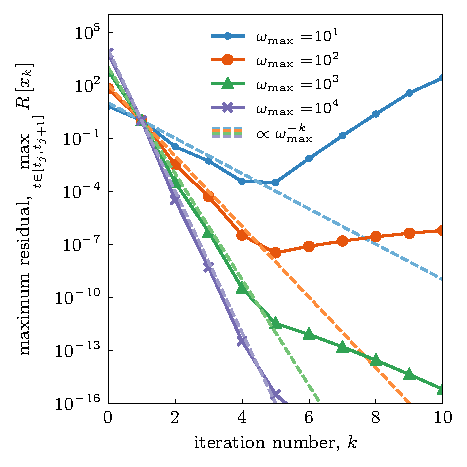
\includegraphics{plots/residual-k-corr.pdf}}
    %\label{residual-reduction}
    \subfloat{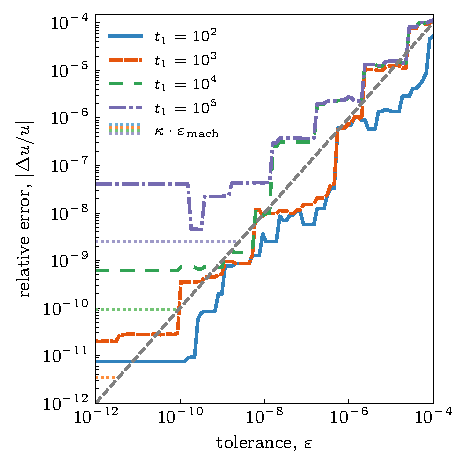
\includegraphics{plots/convergence.pdf}}
    \caption{\label{convergence-plot}
      Demonstrations of Riccati residual defect correction (left plot), and error performance of the overall solver (right plot).
      In detail, the left plot shows the maximum magnitude of the residual
      of the Riccati ODE \cref{R} over the
      $n=16$ Chebyshev grid, as a function of iteration count,
      for the example in \cref{demo}.
      For small $\om_{\text{max}}$ an initial geometric decay eventually becomes
      unstable growth for large $j$. The dotted lines show $\om_{\text{max}}^{-j}$.
      %
      The right plot shows the achieved relative error of the solver against the supplied tolerance for the example in \cref{airy-demo}, while the upper end of the integration interval is varied. The dotted lines show the maximum possible accuracy for each interval as per \cref{conditionnodef}, which the solver indeed achieves to within about one digit.
      %     
   %   Demonstration of residual reduction
 %     Error analysis and convergence of our
 %   method. The left panel shows the maximum residual of the Riccati equation
 %   over a single step of the numerical method as a function of the number of
 %   terms added to the asymptotic expansion, which is used to propagate the
 %   numerical solution in the highly oscillatory regions of the ODE. The
 %   differently coloured curves correspond to different peak frequencies over
 %   the same time interval. A geometric reduction in the residual for the first
 %   few iterations, forecast qualitatively in \cref{phasefun} and shown formally in
 %   \cref{TR}, is observed. Following this geometric reduction the
 %   asymptotic nature of the approximation is manifest as an increase in the
 %   residual, especially visible at low $\omega_{\text{max}}$. The right panel
 %   is a convergence plot showing the achieved relative error against the
 %   relative tolerance set to the solver. The coloured curves correspond to
 %   different upper ends of the integration region. These should be compared to
 %   the grey dashed line showing an achieved error matching the tolerance.
 %   In regions where the condition number $\kappa$ of the problem may limit the achievable
 %   accuracy (see \cref{conditionnodef}), we plot the maximum achievable
      %   accuracy as a coloured dashed line to compare the achieved error with.
      }
   % Need to say what ODEs were used to create these  
\end{figure*}    



\subsection{Matching Riccati timestep intervals}
%\AB{short but probblay seperate subsec like this, since confusing before
%  the demo of Fig.1}

So far we have explained how to numerically solve for 
one approximate nonoscillatory Riccati phase function over one timestep
$[t_i,t_i+h]$,
in the sense of having uniformly small residual on its spectral grid.
% AB note narrative guide.
However, this cannot match general initial conditions
$u(t_i)$ and $u'(t_i)$, as needed for a second order ODE timestepper.
Yet, the asymptotic iteration \cref{iter} can be
initialised with $x_0(t) = +i\om(t)$ (as done in \cref{init}), or with $x_0(t)
= -i\om(t)$. The two resulting Riccati solutions, $x_{\pm}(t)$,
give two linearly independent approximate solutions of the desired ODE
\cref{ode}, namely
\be
u_{\pm}(t) = e^{\int_{t_i}^t x_{\pm}(\sigma)\d\sigma}.
\label{upm}
% *** AB fixed typo here
\ee
Since $\om$ and $\gamma$ are real, $u_{+}$ and $u_{-}$ are complex conjugates.
% AB *** please check this!
% FA: Checked, this statement is correct. Also clarified what 'they' was referring to.
They may be linearly combined to match any set of complex-valued
initial conditions,
\begin{align}
    u(t) &= A_{+}u_{+}(t) + A_{-}u_{-}(t), \qquad t \in [t_i, t_i + h],\\
    u'(t) &= A_{+}u'_{+}(t) + A_{-}u'_{-}(t), \qquad t \in [t_i, t_i + h],
\end{align}
with coefficients $A_\pm$ satisfying the $2\times 2$ linear system
\be
\begin{bmatrix}
    1 & 1 \\
    x_{+}(t_i) & x_{-}(t_i)
\end{bmatrix}
\begin{bmatrix}
    A_{+} \\
    A_{-}
\end{bmatrix}
= 
\begin{bmatrix}
    u(t_i) \\
    u'(t_i)
\end{bmatrix}.
\ee
Here we used that $u_{\pm}(t_i) = 1$ and $u'_{\pm}(t_i) = x_{\pm}(t_i)$ by construction of \cref{upm}.




\subsection{Direct spectral solution on nonoscillatory intervals \label{chebysteps}}

If the solution is nonoscillatory, or the asymptotic expansion fails to
converge before the residual reaches a user-specified tolerance $\varepsilon$, the solver switches to a standard spectral collocation method on a Chebyshev grid.
This achieves an arbitrarily high order timestep in a simple manner.
(We note that in other applications a \emph{global} spectral grid is
advantageous \cite{tref}; here, since adaptive switching and efficiency are
needed,
integration is best performed over many timestep intervals with a fixed high
order grid on each.)
%The motivation
%behind this choice is that by adjusting the number of nodes, an arbitrarily
%high order can be achieved.
%Although spectral methods are usually used for
%solving boundary value problems whereby the nodes are laid out over the entire
%integration range, there is no reason one could not apply them over one timeste%p at a
%time in a time-stepper setting. Since the present algorithm was constructed to
%switch between two methods -- one based on the asymptotic expansion of the
%Riccati equation and a spectral method -- on the fly and the points of
%switching are not predetermined, we opt to break the integration range up into
%smaller timesteps, applying the spectral method over a single timestep at a
%time.
% AB: although I liked some of this story, it was a bit long-winded.
% FA: :(, but I agree.
% And piecewise spectral is a standard idea, not a new one.
%
Using the
Chebyshev nodes $\{\tau_l\}_{l=0}^n$ and differentiation matrix $D_n$
from \cref{discr},
\cref{ode} may then be discretized over the interval $t \in [t_i, t_i+h]$ by
the linear system
\begin{align}\label{discreteode}
  F_n \mbf{u} := \left(D_n^2 + 2\text{diag}(\{\g_l\})D_n + \text{diag}(\{\om_l^2\}) \right)\mbf{u} = \mbf{0},
 % note vector 0. note fixed typo om -> om^2
\end{align}
% AB: again, u_n notation ambgious since it means u at the last node l=n.
where $\mbf{u}:=\{u(\tau_l)\}_{l=0}^n$ is the node value vector, and
% FA: Is node value a standard term? I corrected it earlier...
diag indicates the diagonal matrix constructed from a vector.
One must also enforce initial conditions via
\be\label{discreteic}
u_n
% AB *** why was (u_n)_n here? did you mean (u_n)_0 in your notation?
% FA: No, that was deliberate because the Cheby nodes are ordered backwards
% from 1 to -1 in our notation! Changed it back to how it was.
= u(t_i), \qquad \left(D_n\mbf{u}\right)_n = u'(t_i).
\ee
%where a lower index outside brackets denotes a given vector element. <- AB good but I already did this in sec 2.2 now.
Stacking these conditions as rows gives the overdetermined $(n+3) \times (n+1)$ linear system
\be\label{discreteodeic}
\renewcommand*{\arraystretch}{1.25}
\begin{bmatrix}
    (F_n)_{00} & \ldots & (F_n)_{0n} \\
    \vdots & \ddots & \vdots \\
    (F_n)_{n0} & \ldots & (F_n)_{nn} \\
    (D_n)_{00} & \ldots & (D_n)_{0n} \\
    0 & \ldots & 1
    % AB: note last row is ambiguous. A 2x2 block notation may be easier and
    % shorter
    % FA: Noticed that last row of this system was inconsistent with our Cheby node ordering, so corrected it.
\end{bmatrix}
\mbf{u} =  
\begin{bmatrix}
0 \\
\vdots \\
0 \\
u'(t_i) \\
u(t_i)
\end{bmatrix},
\ee
which is solved in the least-squares sense via SVD with $\bigO(n^3)$ cost.
% AB *** please check - we need to say how.
% FA: Used numpy.linalg.lstsq. After some digging, this calls LAPACK's dgelsd or zgelsd depending on real or complex, which in turn use SVD.
$u(t)$ at the interval's upped end can be read off as the first element of the
solution vector $\mbf{u}$, and its derivative as the first element of
$D_n\mbf{u}$.
% FA: For same reason as above, last -> first
These then serve as the initial conditions for the subsequent time-step.
(Note that square systems may also be created by removing rows \cite{tref}.)
% *** AB is that true? in the narrative you have to state what we did,
% not leave it ambiguous what we did.
% FA: I'm not sure if that's true. If more Cheby steps are required, it may
% become a limiting factor, but for the highly oscillatory problems I profiled,
% this was of course not the bottleneck. I therefore removed the statement
% referring to the speed difference.
%Note that the system has now become rectangular but also overdetermined. The
%matrix on the right-hand-side of \cref{discreteodeic} may be replaced with a
%square one by removing the last two rows and incorporating the initial
%conditions directly, \eg the last row can be removed by solving only for
%$(u_n)_1, \ldots, (u_n)_n$ and setting $(u_n)_0 = u(t_i)$.

We estimate the error induced over this timestep $[t_i,t_i+h]$
by comparing to the solution at the interval endpoint using a doubled value
of $n$.
If the
absolute
% *** AB? relative or abs?
error falls below the user-specified
threshold $\varepsilon$, the step is accepted.
% *** AB which value is used, the original n or the doubled n one?
If the error does not reach $\varepsilon$ by $n=n_{\text{max}}$, $h$
% *** AB I don't understand this: all you have run is n and 2n, so how
% do we get to nmax.? You do not describe an iteration here.
% Since 64^3 is big, I suggest you stick to 16 and 32, then half h if
%
is halved and the iteration in $n$ begins again starting with
$n=n_{\text{min}}$. The parameters $n_{\text{min, max}}$ can be chosen by the
user, but their default values are set to $n_{\text{min}} = 16$,
$n_{\text{max}} = 64$. Computation time spent in failed steps is lost, making
it imperative that the initial stepsize estimate $h$ is chosen carefully. We
describe the procedure for choosing $h$ for both spectral and asymptotic steps
in detail in the next section.
% AB good narrative end!

*** TO TRY FIX n=16,32,64 to n=16,32 only - or describe how decision
to go to 64 is done.





\subsection{Adaptive selection of interval size and type}
\label{adap}

In this section we explain the adaptive stepsize and method-switching
algorithm. The left side of \cref{balls-flowchart} shows
a summary flowchart.

\subsubsection{Initial stepsize estimates}
\label{hosc}

At each timestep start $t_i$, a decision needs to be made about whether to
use the Riccati defect correction or the Chebyshev spectral method.
Both types of steps could be attempted
% simultaneously <- AB they are not simultaneous unless you're doing some
% weird parallel proc model. Trying to get you to be as precise as possible :)
% The reader will thank us.
and the decision based upon the their estimated error (as done in \cite{agocs2020efficient}).
Instead, we find it more efficient to use local properties of $\om$ at $t_i$
to get initial stepsize estimates.
Recalling \cref{x1R1}, the first correction term is $\om'/\om$, giving the
approximate timescale
\be\label{hoscini}
h_{\text{osc}} = \frac{\om(t_i)}{\om'(t_i)}.
\ee
\cref{TR} will also support this by showing that
the ratio of bounds on $\om'$ and $\om$ appears in the rate of
convergence of successive Riccati residuals.
In practice to approximate $\om'(t_i)$, we use Chebyshev differentiation
from the grid of the previous timestep, and from the grid of an initial
stepsize at $t=t_0$, supplied by the user.

% AB note how I'm trying to remove repetition, speculation,
% and keep it to the point.

A similar estimate for the spectral method should depend on two things: how
oscillatory the solution is, and on what timescales the coefficients in \cref{ode} change, \ie their smoothness. Using the former as our criterion,
a measure of the rate of
oscillations is simply the frequency, giving the timescale
\be\label{hsloini}
h_{\text{slo}} = \frac{1}{\om(t_i)}.
\ee

These initial stepsize estimates are too crude to use directly, since
$\om$, $\om'$, or $\g$ may change significantly over such an interval.
Nonetheless they provide a useful starting point for the algorithm that computes
finer estimates.
% AB *** why doesn't eps enter into either of these h estimates?
% FA: eps enters in the stepsize refinement phase -- for the initial estimate I
% just needed a quick and dirty way of estimating the relevant timescales
% without querying \om, \g too many times.
% FA: Also added the (not very sophisticated) way of getting w' at t = t_0 (the start of the solution interval).


\subsubsection{Refining the stepsize estimates}

%The local error of of the asymptotic solution described in \cref{phasefun} is not
%inherently dependent on the stepsize $h$ in the same way a \eg Runge--Kutta
%method's is.
% AB *** note RK would also have prefactors infront of O(h^4) that depend on
% the coeffs, their derivs, etc. So it is no different. Also try reading your
% sentence :)
%
%The convergence rate of the residual of asymptotic steps depends
%on the bounds on $\om$, $\om'$, and $\g$ over the course of the step as we show
%in \cref{TR}, which indirectly introduces stepsize-dependence, as does the fact
%that the derivatives and integral appearing in the step are computed
%numerically on an $(n+1)$-point Chebyshev grid (with $n \approx 16$). Ultimately,
% AB I found the above rambling. The below is a more direct statement:

The discretization used in the Riccati defect correction method in \cref{discr} is certainly no more accurate than
the error in which the coefficient functions $\om$ and $\g$ are represented
on the Chebyshev grid.
%degree Chebyshev polynomials that determines the error in asymptotic steps, which
Therefore we estimate their Chebyshev interpolation error as follows.
Let $\mbf{f}\in\R^{n+1}$ indicate the vector of nodes values
$\{f(\tau_l)\}$ for a function $f$ which will be either $\om$ or $\g$.
Let $f^\star(t)$ be the Lagrange polynomial interpolant through the
nodes $\{\tau_l\}_{l=0}^n$.
Let $\tau^\star_l := t_i + \tfrac{h}{2}[1 + \cos(l\pi/n + \pi/(2n)]$, $l=0,\dots,n-1$ be the set of $n$ points that lie halfway in between the $n+1$ Chebyshev nodes on the unit half-circle.
Then define the error estimate
\be
    \Delta_n[f] := \max_{l = 0, 1, \ldots, n} \biggl| \frac{f(\tau^{\star}_l) -
    f^{\star}(\tau^{\star}_l)}{f(\tau^{\star}_l)} \biggr|,
\ee
where $f$ is $\om$ or $\g$.
In fact $\{f^{\star}(t^{\star}_l)\} = L_n \mbf{f}$ for some interpolation matrix
$L_n$ that is independent of the interval choice, so in practice
$L_n$ is computed only once, by solving a Vandermonde system in a backwards
stable fashion. Even though the system is exponentially ill-conditioned in $n$,
the interpolation itself is very accurate if the underlying function is
sufficiently smooth and Chebyshev (or Legendre) nodes are used. For details,
see \cite[Appendix A]{helsing_close}.
% AB *** either we explain this and cite Helsing appendix and my prior work,
%  or we just say its done by barycentric formulae and cite Berrut-Tref.
%  You decide.
% FA: Finally found the reference for this!

Letting $\Delta$ denote the larger of $\Delta_n[\om]$ and $\Delta_n[\g]$, we accept or update the stepsize as follows,
\be
  %    \Delta :=& \max \left(\Delta_n[\om], \; \Delta_n[\g]\right), \\
  % AB: not sure that deserves a separate formula, esp since want look simpler
    h \leftarrow \begin{cases}
        h &\text{if } \Delta \leq \varepsilon_h, \\
        \min \left( 0.7h, 0.9 h \left( \frac{\varepsilon_h}{\Delta} \right)^{\frac{1}{n+1}} \right) &\text{otherwise},
    \end{cases}
    \ee
    % AB got here
where $\eps_h$ is a parameter quantifying relative tolerance (separate from $\eps$). In the above, the $1/(n+1)$ in the exponent is justified by noting that the
error in ($n+1$)-point Chebyshev interpolation is proportional to $h^{n+2}$, therefore if
$\Delta$ exceeds $\varepsilon_h$, using an exponent slightly larger than $1/(n+2)$ takes
the local error back down to a value smaller than $\varepsilon_h$, which is further
ensured by multiplying by the safety factor 0.9. We decrease the step to $0.7h$
if it yields a smaller stepsize to ensure quicker convergence if $\Delta$ is
only slightly larger than $\varepsilon_h$. The factors 0.7 and 0.9 were set based on
empirical observations. 

The local error of Chebyshev spectral steps depends on both the stepsize and
the number of nodes. Since within a step we iterate over both of these until
convergence, we only need to ensure that over our proposed stepsize the
timescale over which $u$ changes ($\approx 1/\om$) does not increase too much. Starting from $h =
h_{\text{slo}}$, we refine the stepsize proposal according to
\begin{align}
    h :=& \begin{cases}
        h/2 &\text{if } \min\limits_{j = 0, 1, \ldots, n}\frac{1}{\om(t^{\star}_j)} < \sigma h \\
        h &\text{otherwise},
    \end{cases}
\end{align}
with $\sigma = 0.8$, chosen experimentally, and $n$ being a
%hyperparameter  <- AB only stats has hyperparams :)
parameter with a default value of $n = 16$.

\subsubsection{Choosing the step type}
\label{steptype}

With a refined $h_{\text{osc}}$ and $h_{\text{slo}}$ in hand, we can make an informed decision about which type of step to take.
\begin{pro}\label{steptypechoose}
    Let $h_{\text{osc}}$ and $h_{\text{slo}}$ be the refined stepsize proposals
    for a step to be taken from $t = t_i$ using the asymptotic expansion and the Chebyshev
    spectral method, respectively. The algorithm chooses to attempt an
    asymptotic step of size $h_{\text{osc}}$ if and only if
$$ h_{\text{osc}} > 5h_{\text{slo}} \quad \text{and} \quad \omega(t_i) h_{\text{osc}} > 2\pi, $$
    otherwise it will attempt a spectral step of size $h_{\text{slo}}$.
\end{pro}
The reason behind requiring the proposed stepsize for an asymptotic step not to
simply be larger than that of a Chebyshev spectral step is that in regions
where the two stepsizes compete, the asymptotic method rarely converges before
the residual reaches $\varepsilon$, either because $\om$ is not large enough, or
either of $\g$ and $\om'$ is too large. The prefactor of $5$ was set based on numerical experiments. 

If an asymptotic step was decided to be attempted, the algorithm will start
iterating over $x_j$ according to \cref{iter}, monitoring the residual
$R[x_j](t_n)$ throughout. If $\max R[x_j](t_n) < \varepsilon$ \emph{or} $\max
R[x_j](t_n) \geq \max R[x_{j-1}](t_n)$, the iteration is stopped. In the former
case, the proposed solution $u(t_i+h)$ is accepted and the independent variable
is incremented, $t := t_i + h$. Otherwise, the step is re-attempted with size
$h = h_{\text{slo}}$ and using the spectral method. 

If either of the conditions in \cref{steptypechoose} were not met, a spectral
step is attempted with $h = h_{\text{slo}}$. The local error of the step is
then estimated and the number of nodes, as well as the stepsize, is
adapted until a local error value of at most $\varepsilon$ is reached, as described in
\cref{chebysteps}.

A flowchart showing how estimating the stepsizes and choosing the step type ties
together is shown in the left panel of \cref{balls-flowchart}.


\section{Error analysis for the Riccati iteration\label{errorana}}

Here we prove our main rigorous result:
the defect correction of \cref{phasefun}
in the case of analytic coefficients induces
temporary geometric decrease of the Riccati residual by a factor $\bigO(\om)$ per iteration.
%up to a certain number of iterations.
Indefinite geometric decrease is not in general possible because of
factorial growth due to repeated differentiation;
the iteration is asymptotic in $\om\gg 1$, but not convergent.
We abbreviate the residual function by $R_j = R_j(t) := R[x_j](t)$.
Our main tools in proving the following will be \cref{PRiter} (the iteration for $R_j$), induction, and complex analysis.

%For smooth $x_j$ of size $\bigO(\om)$, and smooth $R_j$,
%it suggests geometric reduction in $R_j$ by a factor $\bigO(\om)$ per iteration;
%however, this is misleading in general because of
%growth of high-order $t$-derivatives.
%The series will turn out to be merely asymptotic in the large parameter $\om$.
%We now make this argument rigorous, for $\om$ analytic
%and sufficiently large throughout some neighborhood of $t$.

%One might hope that, given $x_j'$ and $x_j$ of order $\om$,
%and a lower bound on $x_j$ of the same order,
%then $R_j$ is reduced at each point by a factor $\bigO(\om)$.
%then the last term is negligible
%then if $R_j$ and $R_j'$ are sufficiently small

\begin{thm}\label{TR}   
  Fix $t\in\R$, and let the frequency function $\om$ and damping function $\g$ be analytic
  in the closed ball $B_\rho(t) := \{z\in\C : |z-t| \le \rho\}$,
  for some $\rho>0$, with the bounds in this ball
    \begin{alignat}{4}
        \eta_1 \leq \; &|\om(z)| && \leq \eta_2,          \label{ommag} \\
         &|\om'(z)| &&\leq \eta_3 \leq \frac{\eta_1^2}{17}, \label{omder} \\
         &|\g(z)| &&\leq \eta_4 \leq \frac{\eta_1^2}{34\eta_2}. \label{gammaupper}
  \end{alignat}
  %\forall z\in B_\rho(t),
% AB: not sure why you left this in:  "that is, its derivative should be sufficiently small." since there is gamma and omega.
  Let the nonnegative integer $k$ be small enough that
  \be
    r := \frac{1}{2\te_1 \rho} \left(1 + \frac{\te_2}{\te_1}\right) k + \frac{\te_3}{4\te_1^2} \leq \frac{3}{4},
  \label{r}
  \ee
  where
    \begin{align}
    \te_1 &= \eta_1 - \eta_4 - \frac{17 \te_3}{4 \eta_1},  \label{eta1} \\ 
    \te_2 &= \eta_2 + \eta_4 + \frac{17 \te_3}{4 \eta_1},   \label{eta2} \\
    \te_3 &= \eta_3 + 2\eta_2\eta_4. \label{eta3}
    % AB decided ordering 1,2,3 trumps fact that 1,2 depend on 3.
    \end{align}
  Then after any number $j\le k$ of iterations of \cref{init}--\cref{iter},
  the function $x_j$ has Riccati residual \cref{R} bounded at the point $t$ by
  \be
  |R_j(t)| \le \te_3 r^j. \label{Rjbnd}
  \ee
\end{thm}  % ttttttttttttttttttttttttttttttttttttttttttttttttttttttttttttt

\begin{figure*}[tb]
    \centering
    \subfloat{\begin{adjustbox}{width=0.45\textwidth, valign=c}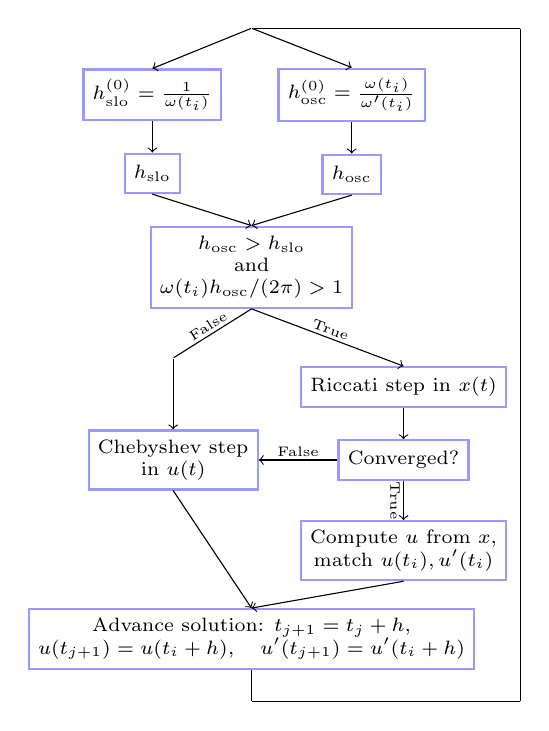
\begin{tikzpicture}[ roundnode/.style={circle, draw=black!60, fill=green!0, very thick, minimum size=7mm}, squarednode/.style={rectangle, draw=blue!40, fill=red!0, thick, minimum size=5mm}]

\tikzstyle{every node}=[font=\scriptsize]

%Nodes
\node[squarednode]      (hsloini)   {$h_{\text{slo}}^{(0)} = \frac{1}{\omega(t_i)}$};
\node[squarednode]      (hoscini)  [right=0.7cm of hsloini] {$h_{\text{osc}}^{(0)} = \frac{\omega(t_i)}{\omega'(t_i)}$};
\node[squarednode]      (hslo)  [below=0.4cm of hsloini] {$h_{\text{slo}}$};   
\node[squarednode]      (hosc)  [below=0.4cm of hoscini] {$h_{\text{osc}}$};    
\node[squarednode, align=center]      (switch) [below right=0.4cm and -0.4cm of hslo] {$h_{\text{osc}} > h_{\text{slo}}$ \\ and \\$\omega(t_i) h_{\text{osc}}/(2\pi) > 1$};
\node[squarednode]      (ricc)  [below right=3.1cm and -1.6cm of hoscini] {Riccati step in $x(t)$};  
\node[squarednode]      (conv)  [below=0.4cm of ricc] {Converged?}; 
\node[squarednode, align=center]      (cheb)  [left=1cm of conv] {Chebyshev step \\ in $u(t)$}; 
\node[squarednode, align=center]      (ic)  [below=0.5cm of conv] {Compute $u$ from $x$, \\ match $u(t_i), u'(t_i)$};     
\node[squarednode, align=center]      (accept)  [below =3.8cm of switch] {Advance solution: $t_{j+1} = t_{j}+h$, \\ $u(t_{j+1}) = u(t_i + h), \quad u'(t_{j+1}) = u'(t_i + h)$ };    
%\node[inner sep=0, minimum size=0, below left=0.7cm and -0.05cm of switch] (k) {}; % invisible node
\node[inner sep=0, minimum size=0, above=0.9cm of cheb] (k) {}; % invisible node
\node[inner sep=0, minimum size=0, below=0.4cm  of accept] (l) {}; % invisible node
\node[inner sep=0, minimum size=0, right=3.4cm of l] (m) {}; % invisible node
\node[inner sep=0, minimum size=0, above=2.5cm of switch] (o) {}; % invisible node
\node[inner sep=0, minimum size=0, right=3.4cm of o] (n) {}; % invisible node   

%Lines
\draw[->] (hsloini.south) -- (hslo.north);
\draw[->] (hoscini.south) -- (hosc.north);
\draw[->] (hosc.south) -- (switch.north);
\draw[->] (hslo.south) -- (switch.north);
\draw[->] (switch.south) -- (ricc.north) node[midway, above=-0.5ex, sloped] {\tiny True};    
\draw[-] (switch.south) -- (k) node[midway, above=-0.5ex, sloped] {\tiny False};  
\draw[->] (k) -- (cheb.north) ;
\draw[->] (conv.south) -- (ic.north) node[midway, below=-0.5ex, sloped] {\tiny True};    
\draw[->] (conv.west) -- (cheb.east) node[midway, above=-0.5ex] {\tiny False};
\draw[->] (ic.south) -- (accept.north); 
\draw[->] (cheb.south) -- (accept.north);    
\draw[->] (ricc.south) -- (conv.north);
\draw[-] (accept.south) -- (l) ;
\draw[-] (l) -- (m) ;    
\draw[-] (m) -- (n) ;    
\draw[-] (n) -- (o) ; 
\draw[->] (o) -- (hsloini.north) ;
\draw[->] (o) -- (hoscini.north) ;    

\end{tikzpicture}
\end{adjustbox}}
    \hfill
    \subfloat{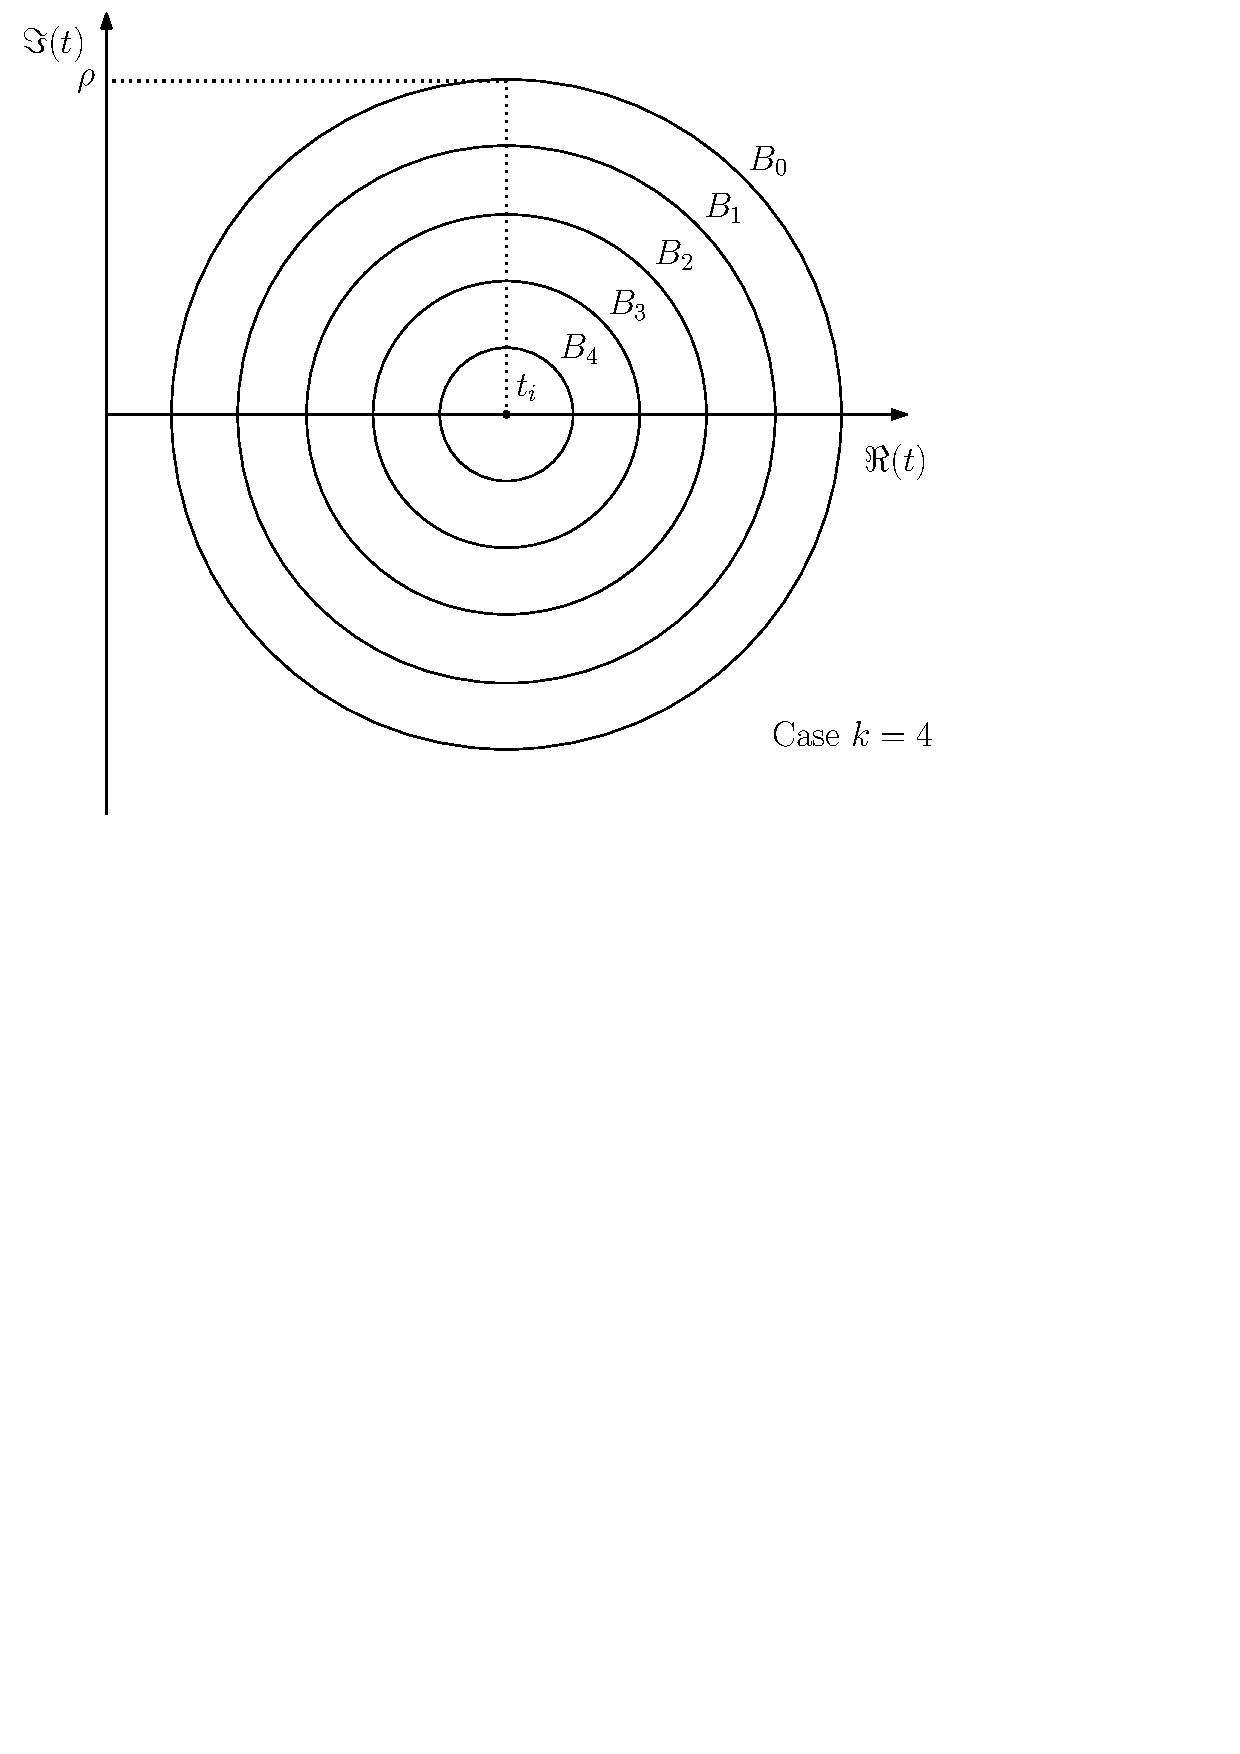
\includegraphics[width=0.5\textwidth, valign=c]{plots/complexsetup.pdf}}
    \caption{\label{balls-flowchart} Left: Flowchart showing choice of stepsize $h$ and step type (Riccati vs standard Chebyshev) for our proposed algorithm.
      $t_i$ is the start of the current timestep.
    Right: Sketch of a nested equispaced set of
      balls centered on the target time $t$, used in the proof of \cref{TR}.}
\end{figure*}

This shows, for $\om'$ and $\g$ sufficiently small,
temporary geometric convergence up to $k$ iterations,
but at a rate $r$ that deteriorates with $k$.
For any $k$ to satisfy \cref{r}, $\om$ must have
a sufficiently large lower bound $\eta_1$, \ie $t$
must be in a sufficiently oscillatory region for the original ODE.
The condition \cref{omder} on $\om'$ is similar to
that in WKB: the \emph{relative $\om$ change per period} should be less than some small constant.

\begin{rmk}\label{slight}
  By construction, $[\te_1,\te_2]$ is only a limited
  expansion of the interval $[\eta_1,\eta_2]$ containing the range of $|\om|$ in the ball.
  In particular, by the inequalities \cref{ommag}--\cref{gammaupper} and
  definitions \cref{eta1}--\cref{eta3},
  % AB: cref actually failed here; I prefer eqref anyway.
  % FA: Sorry, but changed it to cref (it works now)... I much prefer cref.
  $\te_1 \ge 8\eta_1/17$ and $\te_2 \le \eta_2 + 9\eta_1/17$.
  Applying this we see that the last term in the definition of $r$ in \cref{r}
  is no more than $17/128 \leq 0.14$, thus can at worst cause only modest
  deterioration in the rate.
\end{rmk}

\begin{rmk}
  In the limit when $\om$ tends to be constant in the ball ($\eta_3$ small) and damping is small ($\eta_4$ small),
  then the geometric rate $r$ tends to $k/\om \rho$, where we can interpret $\om\rho$ as $2\pi$
  times the number of oscillation periods across the ball radius.
  Then, for example, with a radius of only 5 periods, $r$ satisfies \cref{r}
  for $k\le 25$.
\end{rmk}

\begin{proof}
  Define the concentric nested set of closed balls $B_j := B_{\rho_j}(t)$,
  with radii $\rho_j := (1-j/k)\rho$, $j=0,1,\dots,k$. Note that
  $B_0$ is the original ball in the statement of the theorem, while
    $B_k = \{t\}$ is the single point of interest; see the
    right panel of \cref{balls-flowchart}.
  For any function $f$ analytic in $B_j$ we abbreviate its $\infty$-norm by
  $\|f\|_j := \max_{z \in B_j}|f(z)|$.
  We will bound $f'$ in $B_{j+1}$ in terms of $\|f\|_j$ by
  applying Cauchy's theorem for derivatives
  \cite{steinshakarchi},
  \be
  f'(z) = \frac{1}{2\pi i} \int_{|\zeta-t|=\rho_j} \frac{f(\zeta)\, d\zeta}{(\zeta-z)^2}, \qquad z \in B_{j+1}.
  \label{cauder}
  \ee
  Bounding the integrand, then using the cosine rule we get
  $$
  |f'(z)| \le 
  \frac{\|f\|_j}{2\pi} \int_{|\zeta-t| = \rho_j} \frac{|d\zeta|}{|\zeta-z|^2}
  =
  \frac{\|f\|_j}{2\pi} \int_0^{2\pi} \frac{\rho_j\, d\theta}{|z|^2 + \rho_j^2 - 2|z|\rho_j \cos \theta}.
  $$
  We now use $\int_{0}^{2\pi} d\theta /(a + b \cos \theta) = 2\pi/\sqrt{a^2-b^2}$
  for $b<a$ \cite[Eq.~3.613.1]{GR8}, with
  $a = |z|^2 + \rho_j^2$ and $b = -2|z|\rho_j$, so that
  $\sqrt{a^2-b^2} = \rho_j^2-|z|^2$.
  Noting that the case $|z| = \rho_{j+1}$ bounds the others,
  and using $\rho_j=(1-j/k)\rho$, we compute, for any $0\le j < k$,
  \be
  \|f'\|_{j+1} \le
  \frac{\|f\|_j}{2\pi} \frac{2\pi\rho_j}{\rho_j^2-\rho_{j+1}^2}
  =
  \frac{\|f\|_j}{2 \rho} \frac{k(k-j)}{2k-2j-1}
  =
  \frac{\|f\|_j}{2 \rho} k \left[ \frac{1}{2} + \frac{1}{2(2k-2j-1)}\right]
  \le
  \frac{k}{\rho}\|f\|_j.
  %~, \; 0\le j< k
  \label{derbnd}
  \ee
  Note that this bound is a factor $\bigO(k)$ better than naively
  lower bounding the denominator in \cref{cauder}.
  
  %The 
  We now use induction in iteration number $j$.
%  and consider the iteration acting on the functions
    We take as the induction hypothesis that $x_\ell$ (and thus $R_\ell$)
  is analytic in $B_j$, for all $0\le \ell \le j$, with
  \begin{align}
      \te_1 \leq |x_\ell + \g| &\leq \te_2
  \qquad \mbox{ in } B_j, \quad \mbox{ for all } \ell = 0,1,\dots,j,
  \label{hypx} \\
      |R_\ell| &\leq \te_3 r^\ell \quad \mbox{ in } B_j, \quad \mbox{ for all } \ell = 0,1,\dots,j,
  \label{hypR}
  \end{align}
  where $r$ is defined by \cref{r}.
  Assuming for now the hypothesis for $j$, we apply simple bounds to the
  residual iteration \cref{Riter},
  lower-bounding denominator magnitudes and upper-bounding numerators
  via \cref{hypx},
  and applying \cref{derbnd} to the two derivative terms, to get
  $$
  \|R_{j+1}\|_{j+1}
  \leq
  \frac{1}{2\te_1}\left(
  \frac{1}{\te_1} \frac{k}{\rho}\te_2 + \frac{k}{\rho}
  \right)\|R_j\|_j
  +\biggl(\frac{\|R_j\|_j}{2\te_1}\biggr)^2
  \leq
  r \cdot \|R_j\|_j
  \leq
  \te_3 r^{j+1},
  $$
where in the middle step we used the crude bound $\|R_j\| \le \te_3$
following from \cref{hypR} and that $r\le1$, and then the definition of $r$ in \cref{r}.
%This handles the case $\ell=j+1$.
The lower cases $\ell\le j$ follow trivially from the hypothesis since the balls
are nested.
Thus \cref{hypR} is proven for $j+1$.

It remains to verify that \cref{hypx} also holds for $j+1$.
By the functional iteration \cref{init}--\cref{iter},
$$
x_{j+1}(z) + \g(z) = i\om(z) + \g(z) - \sum_{\ell=0}^{j} \frac{R_\ell(z)}{2 \left(x_\ell(z) + \g(z)\right)},
\qquad z\in B_{j+1}.
$$
Using the hypothesis, the sum is pointwise bounded in magnitude
in $B_{j+1}$ by
$$
\left|\sum_{\ell=0}^{j} \frac{R_\ell}{2\left( x_\ell + \g \right)} \right|
\leq \frac{\te_3}{2\te_1} \cdot \sum_{\ell=0}^j r^{\ell}
%\;\le\; \frac{\eta_3}{2\te_1} \frac{1}{1-r}
\leq \frac{\te_3}{2\te_1} \cdot 4,
%\leq \frac{95\eta_3}{198\eta_1}
$$
where the upper bound in \cref{r} was used to bound the geometric series.
Using \cref{eta1} for $\te_1$ and \cref{eta3} for $\te_3$ we write this upper bound as
$$
\left|\sum_{\ell=0}^{j} \frac{R_\ell}{2\left( x_\ell + \g \right)} \right|
\leq
2\frac{\eta_3 + 2\eta_2\eta_4}{\eta_1 - \eta_4 - \frac{17\eta_3}{4\eta_1} - \frac{17\eta_2\eta_4}{2\eta_1}},
$$
then extend it by lower-bounding the denominator via \cref{omder} and the crude bound ${\eta_4 \leq \eta_1/34}$ from \cref{gammaupper}. This gives
$$
\left|\sum_{\ell=0}^{j} \frac{R_\ell}{2\left( x_\ell + \g \right)} \right| 
\leq
\frac{17\eta_3}{4\eta_1} + \frac{17\eta_2\eta_4}{2\eta_1},
$$
which, when combined with $|\om| \leq \eta_2$ and $|\g| \leq \eta_4$ yields
$$\|x_{j+1} + \g\|_{j+1} \le \eta_2 + \eta_4 + \frac{17\eta_3}{4\eta_1} + \frac{17\eta_2\eta_4}{2\eta_1} = \te_2,$$
verifying the upper bound \cref{hypx} for $j+1$.
Instead combining with $|\om| \ge \eta_1$ gives
$$ |x_{j+1}| \ge \eta_1 - \eta_4 - \frac{17\eta_3}{4\eta_1} - \frac{17\eta_2\eta_4}{2\eta_1} = \te_1 $$
in $B_{j+1}$, which verifies the lower bound \cref{hypx}.
Again, the hypothesis is inherited for $\ell\le j$ by the nesting of the balls.

Finally, the base case $j=0$ for induction
satisfies \cref{hypx}--\cref{hypR}
by the conditions of the theorem,
since $x_0(t) = i\om(t)$, noting $[\eta_1,\eta_2] \subset [\te_1,\te_2]$,
while $R_0(t) = i\left(\om'(t) + 2\g\om \right)$ is bounded in magnitude by $\te_3$.
\end{proof}

In the above theorem, the choice of $3/4$ in \cref{r} was merely a convenient one, chosen so that the bounds $[\te_1,\te_2]$ on $|x_j|$
involving the geometric sum were
not much wider than the bounds $[\eta_1,\eta_2]$ on $|\om|$.
%It is possible to write simpler but less tight formulae for $r$.
Note that in the case of $\gamma\equiv 0$ it is possible to
simplify the statement and proof of the theorem somewhat,
and improve some of the constants.


\subsection{Practical aspects of residual reduction \label{pracres}}

The fact that, as $k$ grows,
the rate $r$ bound in \cref{TR} deteriorates, we believe to be
an inevitable consequence of
the series generated by the iteration being asymptotic in $1/\om$ but not in general convergent.
However, given a function $\om(t)$ uniformly large enough
in a ball,
by stopping at a roughly optimal $k$ (an idea
called ``superasymptotics'' \cite{berrysuper,boydsuper})
one can achieve
exponential convergence with respect to the size of the frequency $\om$,
as follows.

\begin{cor}[Superasymptotic approximation]\label{super}
  Suppose $\om$ and $\g$ satisfy the conditions \cref{ommag}--\cref{gammaupper}
  about a point $t\in\R$,
  and let $\alpha := (1+\te_2/\te_1)/2\te_1\rho$ be the
  first term in the rate \cref{r} arising from these bounds.
  Then there is a nonnegative integer $k$ such that
  $$
  |R_k(t)|  \le  e \te_3 e^{-1/5\alpha}.
  $$
\end{cor}
\begin{proof}
  Set $k$ to be the integer in the interval $[1/5\alpha-1, \, 1/5\alpha)$.
    Then since the final term in \cref{r} is bounded by $17/128 \leq 0.14$
    by \cref{slight}, and the
    first term is $k\alpha \le 1/5$, we get $r\le e^{-1}$, which
    is also $\le 3/4$ so that \cref{Rjbnd} holds.
    Choosing $j=k$, and inserting the lower bound on $k$,
    $|R_k(t)| \le \te_3 r^k \le \te_3 e^{-(1/5\alpha-1)}$, which
    finishes the proof.
  \end{proof}
Recalling that $\alpha = \bigO(1/\om)$, this
shows that an $\om$-dependent
number of iterations can give, in exact arithmetic, an
exponentially convergent pointwise residual,
$$
|R(t)| = \bigO(e^{-c\om})
$$
for some constant $c>0$.
In the limit where
$\om$ tends to constant in the ball of radius $\rho$ about $t$, then
$\alpha$ tends to $1/\om\rho$, so the above
constant is roughly $c\approx \rho/3$.
Equivalently, roughly one decimal digit is achieved per
$1.1$ periods of oscillation across the ball radius.
% log(10)*3/(2*pi) = 1.099

However, this optimal number of iterations grows as $k = \bigO(\om)$,
so for large $\om$ is impractical, and unnecessary.
In practice we use the adaptive residual stopping criterion for $k$
described in \cref{steptype}.
%on user-defined tolerance
By returning to \cref{TR} and dropping the small second term
in \cref{r} we get, in the limit of constant $\om$ in the ball,
$$
|R_k(t)|  \approx  \te_3 \left( \frac{k}{\rho\om}\right)^k.
$$
This shows \textit{nearly} geometric convergence in $k$,
sufficient to reach machine accuracy efficiently with a few iterations
when $\om$ is large.
For large $\rho\om$ one may approximately invert this to predict the iteration number $k$ sufficient for $|R_k| \approx \varepsilon$, to get
$ k_\varepsilon \approx \frac{\log \varepsilon^{-1}}{\log \rho\om}$,
a refinement of \cref{fewer}.
%*** compare to numerics.

% AB here
Finally we show that the stopping criterion for $k$ based on the absolute
residual $R[x_k]$ of the Riccati equation is relevant because this is equal
to the \emph{relative residual} of the original ODE.
% AB this is a Prop since it's a short indep result. A Cor is a downstream result depending on a prior theorem.
\begin{pro}[Relationship of residuals]\label{residualu}
    Let $R[x_k](t)$ be the residual of the Riccati equation as defined in
    \cref{R}.
    % after $k$ iterations of \cref{init,iter} <- not part of the statement.
    Then if
    $\tilde{R}[u_k](t)$ is the associated residual of the original ODE
    \cref{ode}, defined as
    \be\label{Rode}
    \tilde{R}[u_k](t) := u''_k + 2\gamma(t)u'_k + \omega^2(t) u_k,
    % note correction of last term
    \ee
    for $u_k(t) = e^{\int_0^t x_k(\sigma)\mathrm{d}\sigma}$, then
    % AB note t needs to be on left if on right
    \be
    \frac{\tilde{R}[u_k](t)}{u_k(t)} = R[x_k](t).
    \ee
\end{pro}
\begin{proof}
    This follows straightforwardly from substitution of the above form of $u_k$ into \cref{Rode}.
\end{proof}



\section{Numerical results \label{numresults}}

% AB: here I simplified, but also realised kappa defs needed thinking out
% a but more, fixing formulae.

Our numerical experiments will test the integration of 2nd-order linear
ODEs that include regions with highly-oscillatory solutions.
In such regions the condition number of the problem itself becomes
large, and this limits the achievable accuracy of \emph{any}
numerical method that works with finite-precision input data.
Recall \cite[Ch.~6]{GCbook}
that the definition of relative condition number for evaluation
of a fixed function $f(t)$ is $\kappa(t) := |tf'(t)/f(t)|$.
As a toy example,
%(see, \eg, \cite[Ex.~6.1.3]{CGbook}),  % for sin x
for the oscillatory function $f_{\omega_0}(t) = e^{i\om_0t}$, 
the condition number of evaluating $f_{\omega_0}(1)$ is $\kappa(1) = \om_0$,
the total phase accrued
%of order the number of oscillations
over the interval $[0,1]$.
However, since $\om_0$ is also an input to this problem,
the relative condition number
\emph{with respect to variation in} $\om_0$ is also relevant.
The latter is
$|\om_0/f_{\om_0}(1)| \cdot |\partial f_{\om_0}(1)/\partial \om_0| = \om_0$,
in this case the same as the condition number with respect to $t$.
Thus, if $\om_0=10^{7}$, so that $\kappa=10^7$ by either %above
definition,
then using double-precision arithmetic with
$\varepsilon_{\mathrm{mach}} \approx 10^{-16}$
no algorithm can achieve an error less than $\bigO(\kappa\cdot \varepsilon_{\mathrm{mach}}) \approx 10^{-9}$,
the error for a backward-stable algorithm.

For more general oscillatory solutions to the IVP \cref{ode}--\cref{ic1},
the two above types of condition number generally differ,
and the larger controls the minimum achievable error.
For example, scaling $\om(t)=\om_0 \Omega(t)$ as in \cref{introduction},
then taking the zero-order approximation
$u(t) = e^{\pm i \om_0 \int_{t_0}^t \Omega(\sigma) \d\sigma}$,
we see that its relative condition number with respect to
$t$ is $|t\om(t)|$, detemined by the local frequency,
whereas with respect to
$\om_0$ it is $\int_{t_0}^t \om(\sigma) \d\sigma$, the total phase
accrued over $(t_0,t)$.
%This linear growth in $\kappa$ with respect to the number of oscillations
%also applies to general oscillatory solutions $u(t)$ for
The loss in achievable accuracy due to the latter $\kappa$
is well known, and may be interpreted as 
inevitable accuracy loss in taking the sine or cosine of the phase function
\cite{bremer2018}.
This motivates the following.
\begin{defn}[Condition number and achievable accuracy for an oscillatory region]
  \label{d:kappa}
  Let $u$ be a solution to \cref{ode} on $(t_0,t_1)$ of the form
  $u(t) = e^{z(t)}$ where $\im z'(t) > 0$ for all $t\in(t_0,t_1)$.
  % ie, fixed sign, so winding can never stop and unwind, which would require
  % instead a BV norm on z, or L1 norm on x.
  We define the condition number of the problem of evaluation of $u(t)$
  by
  \be
  \kappa := \max\left[ \, |tz'(t)|, \, \im \, ( z(t) - z(t_0) )\, \right]
  \label{conditionnodef}
  \ee
  and then the resulting best achievable accuracy using finite precision by
  \be
  \kappa \cdot \veps_{\mathrm{mach}}.   % was confusing to duplicate \veps symbol
  \label{mineps}
  \ee
\end{defn}
In practice we use a numerical phase function solution to estimate $\kappa$.
In our examples the first (frequency) term does not dominate the second (accrued phase) term.
In the case where there is no such global phase function
representation $u=e^z$, 
we estimate this second term
% total unsigned phase accumulated
by summing the absolute differences in $\im z$ across
% AB maybe the unsigned aspect isn't needed if the sign of winding doesn't
% flip. TV norm issue, really.
the various intervals in each of which a local phase function exists.
Note that this definition does not
capture additional $\kappa$ fluctuations inherent in real-valued
functions:
taking the real part of the toy example, $f_{\om_0}(t) = \cos \om_0 t$,
$\kappa$ with respect to $t$ becomes $|t\om_0 \tan \om_0 t|$,
which fluctuates wildly from $0$ to $\infty$,
although a typical value is again $\bigO(\om_0)$.

In the below tests we denote absolute error in a numerical solution by
$\Delta u(t) := |u(t) - \tilde u(t)|$, where
$u$ is a reference solution computed either analytically
or by a convergence reference solver,
% FA: *** convergence -> convergent reference solver?? Is this a term usually used?
and $\tilde u$ is the solution given by the method under test.

All computations were performed on an Intel Xeon Gold 6244,
16-core, 3.6 GHz workstation with 264 GB of RAM.
% FA: Seriously, that much RAM?! I got this from cat /proc/meminfo, by looking at the MemTotal field. Yes, nice, right?
The open-source software implementing the proposed method and the above
experiments in \texttt{Python} is available on GitHub\footnote{*** URL HERE}.
The code relies on the \texttt{numpy} \cite{numpy2020} and \texttt{scipy} \cite{scipy2020}
packages to perform linear algebra. For the numerical experiments, the
following versions of software were used: \texttt{Python} 3.8.12,
\texttt{numpy} 1.23.4, \texttt{scipy} 1.9.2.
% FA: *** Python, numpy versions verify  TODO once experiments ran again. 
% AB *** maybe add comment about nothing was paralellized, bascially single-core
% implementations.


\subsection{The Airy equation}\label{airy-demo}

A simple but effective test for highly oscillatory solvers is the Airy ODE,
\be
u'' + tu = 0, \quad t \in [1, 10^8],
\label{airy}
\ee
with initial conditions
\be
u(1) = \text{Ai}(-1) + i\text{Bi}(-1), \quad u'(1) = - \text{Ai}'(-1) -i\text{Bi}'(-1).
\label{airyic}
\ee
where Ai, Bi are the Airy functions \cite[Chapter~9]{DLMFairy}.
Its unique solution is
\be
u(t) = \text{Ai}(-t) + i\text{Bi}(-t).
\ee
%\AB{Good aim to explain why a good test here. I think we need to refine the
%  points though}
It is difficult
%\AB{surely any osc soln is equally bad for std methods?}
for standard numerical methods due to the growing frequency $\om(t) = \sqrt{t}$,
but is expected
to be easy for specialised oscillatory methods since the change in $\om(t)$ per wavelength becomes arbitrarily small, making an asymptotic approximation (such as WKB) 
%-- the zeroth order solution --
an increasingly good local appoximation.
%\AB{We're dancing between a precise and merely intuitive claim here.
%  Maybe rather than state a formula that is not really right since $\om(t)$
%  changes, why not just state in words that the relative
%  change in $\omega(t)$ per wavelength becomes arbitrarily small as $t$ grows?
%  ``Zero order'' sounds precise but I don't think is since what's the expansion, WKB?}
%With this test
%case one can check whether the method adapts its stepsize correctly and
%achieves the maximum possible accuracy, defined in \cref{mineps}.
%\AB{that last point applies to any osc ode, right?}


%\AB{new para since presenting results now}
Choosing a tolerance $\veps=10^{-12}$,
\cref{airy-results} shows the
internal steps our numerical solver takes while solving
\eqref{airy}--\eqref{airyic},
colour-coded by step type, as well as the progression of stepsizes,
the numerical relative error function $\Delta u(t)/u(t)$,
and number of oscillation periods traversed in a single step,
$n_{\text{osc}}$.
The
stepsize $h$ is expected to reflect the timescale over which $\om$ changes,
therefore $h \propto \om(t)/\om'(t) \propto t$, which is observed.
The numerical
error traces the theoretical minimum, $\kappa \cdot \varepsilon_{\text{mach}}$, to
within a digit. The number of oscillations traversed per step can be derived
from $h(t)$: $n_{\text{osc}} \propto \om h \propto t^{3/2}$,
a result clearly supported by the bottom-right figure panel.
% AB don't forget the the summary brag sentence:
Our solver covers around $10^{11}$ periods using ABOUT $10^3$ timesteps ***,
taking *** milliseconds of CPU time,
while achieving an error around $10^{-11}$ (or, when larger, the theoretical
minimum \eqref{mineps}).

%An essential measure of robustness for an adaptive numerical method is convergence, accuracy achieved against accuracy demanded.
The right panel of \cref{convergence-plot} demonstrates the convergence
of our method on the Airy equation for different solution interval lengths,
achieved by varying $t_1$ with $t_0=1$ fixed.
This shows that the achieved relative accuracy is approximately bounded
(within close to one digit of accuracy)
by the requested tolerance $\varepsilon$,
down to the theoretical minimum error \eqref{mineps}.

\begin{figure}[tb]
    \centering
    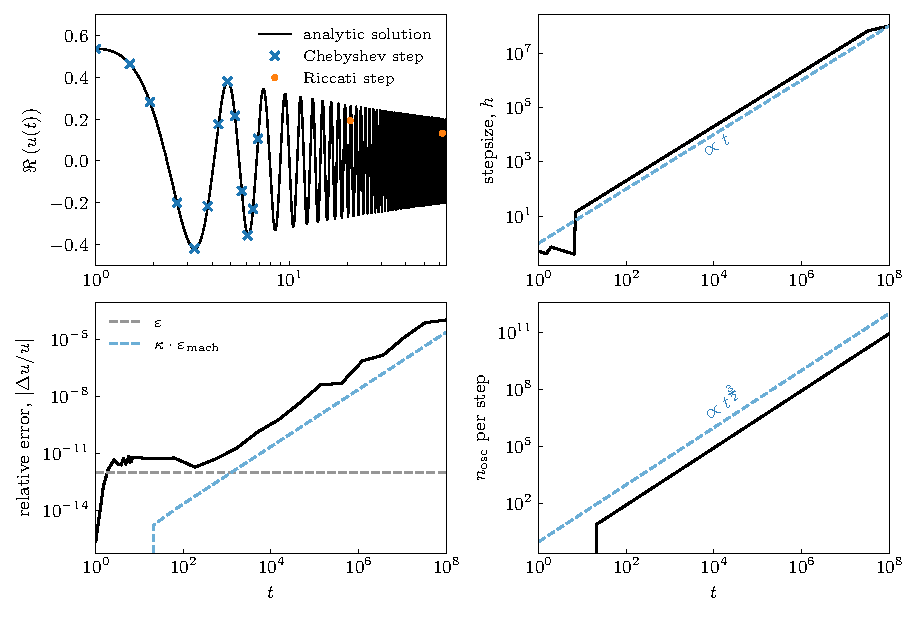
\includegraphics{plots/airy-numsol.pdf}
    \caption{\label{airy-results} Numerical solution of the Airy equation. The
    top left panel shows the real part of the analytic solution in black, on
    top of which the individual timesteps of the solver are plotted, coloured
    by their step type. The top right panel plots the stepsize as a function of
    time, which exhibits linear growth. The bottom left shows the relative
    error achieved by the solver in black, with two dashed lines to guide the
    eye: the chosen solver tolerance $\veps$ in grey, and the
    best achievable accuracy \eqref{mineps}
    in blue. On the
    bottom right, we show the number of wavelengths of oscillation traversed in
    a single step, as a function of time. 
%    This is expected to be roughly proportional to the frequency times timescale over which $\om$ changes, which is $\om^2/\om' = t^{3/2}$, plotted in dashed blue. 
    %, $u'' + tu = 0$, on $t \in [1, 10^8]$, with initial conditions $u(1) = \text{Ai}(-1) + i\text{Bi}(-1)$, $u'(1) = - \text{Ai}'(-1) -i\text{Bi}'(-1)$.   
    }
\end{figure}


\subsection{Comparison with standard and state-of-the-art oscillatory solvers \label{solvercomp}}

Here we compare the performance of the present solver, which
we now refer to as adaptive Riccati defect correction (ARDC), to that of the
following recent specialised methods for oscillatory ODEs:
\begin{description}
\item[Kummer's phase function method:]{ an arbitrarily high-order solver
        described by Bremer \cite{bremer2018}, specifically created for highly
        oscillatory problems with neither a friction term nor
        transitions to nonoscillatory behaviour.
        %operating near machine precision. <- not sure what this means.
        % AB: note criticizing the method before testing is not good here
        % - save it for the Intro, or discussion.
        %Its main
        %drawbacks are the lack of generalisability to include a friction term
        %and to operate at low frequencies or non-oscillatory regions of the
        %solution.
        We use the \texttt{Fortran 90} implementation provided by its author
        at
        \url{https://github.com/JamesCBremerJr/Phase-functions}
        % AB *** how is \om input, since you describe that for oscode below?
        }
\item[oscode:]   % AB sorry gives tex errs for me, will work on
  %\texttt{\textbf{oscode}}
{an adaptive solver which switches from low-order WKB (in oscillatory regions) to Runge--Kutta (in smooth regions)
        \cite{agocs2020efficient,agocs2020dense}, that can accommodate a
        friction term. It requires
        only requires the user to specify $\om$ and $\g$, which can be given as
        either closed-form functions or as timeseries. The solver has both a
        \texttt{Python} and \texttt{C++} interface, but for the experiments below it is called in
        \texttt{Python}.}
\item[The WKB marching method] {\cite{arnold2011wkb,korner2022wkb}:
  a solver using
        the mechanism of \cite{agocs2020efficient} to switch between
        WKB-inspired and Runge--Kutta
        methods. Its convergence order in the oscillatory regions is one higher
        than that of \texttt{oscode}, but does not (easily) generalise to
        include a $\g$ term. It requires the user to provide
        the derivative functions of $\om$ up to $\om^{(5)}$.
%        This recently developed  ... well, all are :)
        It is implemented in \texttt{MATLAB}.
    }
\end{description}

% AB note how I remove extraneous words...
As the test problem we take the ODE in \cite[Eq.~(237)]{bremer2018},
\be\label{bremer237eq}
u'' + \om^2(t) u = 0, \qquad \mbox{ where} \;\; \om^2(t) = \lambda^2(1 - t^2\cos3t)
\ee
on $t \in [-1, 1]$, subject to the initial conditions
\be\label{bremer237ic}
u(-1) = 0, \quad u'(-1) = \lambda,
\ee
where we vary the frequency scaling $\lambda$ between $10^1$ and $10^7$.
% AB consider changing lambda to om_0 throughout, clearer.

For a reference solver we 
use the Kummer's phase function method, since it is arbitrarily high
order, and exhibited around $13$ accurate digits
in its published tests at $\lambda = 10^1$ \cite[Table~1]{bremer2018}.
As expected,
%by Definition~\ref{d:kappa},
the ill-conditioning of the problem as $\lambda$
grows
reduces its accuracy, giving only $8$ digits by $\lambda = 10^7$.
This is in accordance with the theoretical minimum error \eqref{mineps},
thus there will be no meaning given to reported errors below these.
Note that conventional solvers are ruled out as a reference since
the number of oscillations we test are simply too large.

\cref{bremer237tab} presents the runtime statistics of the present method,
\texttt{oscode}, and the WKB marching method, respectively, separated by double
lines. For \texttt{oscode}, the table contains two separate entries that have
been generated with the relative tolerance set to $10^{-6}$ and $10^{-12}$,
respectively. This is reflected in the achieved error in the low-$\lambda$
limit. For all other solvers, we set the relative tolerance to $\veps=10^{-12}$, and
in all cases work in double precision. For our solver, we set the number of
Chebyshev nodes in Riccati (oscillatory) steps (see \cref{chebysteps}) to $n = 40$, the
tolerance for stepsize selection to $\varepsilon_h = 10^{-13}$, and the number
of Chebyshev nodes in the spectral (nonoscillatory) steps to the default
$n = 16$. For \texttt{oscode} and the WKB
marching method none of the parameters were modified from their default values
with the exception of the local tolerance.
% Slightly imprecise as the number of nodes is (n+1) - AB: fine

We now describe the quantities tabulated in \cref{bremer237tab}:
\begin{description}
    \item[$\bm{\mathrm{max}|\Delta u/u|}$:]{Maximum relative error over the
        integration range, evaluated at the timesteps taken internally by the
        solver. If less than the error of the reference Kummer method
    as reported in \cite[Table~1]{bremer2018}, the latter is stated as its upper bound.}
    \item[$\bm{t_{\mathrm{solve}}}$:]{Total runtime, in seconds, of a single
        ODE solve, averaged over between $10^3$ and $10^5$ runs. This is equivalent to the
        ``phase function construction time'' of
        \cite[Table~1]{bremer2018}.
        However, due to different implementations and programming languages,
        this has limited meaning comparing across methods.}
      % AB *** tricky since are you claiming speedups over Bremer, or not?
      % This implies you're not.
      
%    \item[$\bm{t_{\mathrm{eval}}}$:]{Time it takes for the program to evaluate
%        the solution at an arbitrary point other than the internal timesteps.
%        This time should be compared to the ``average phase function evaluation
%        time'' of Table 1 \cite{bremer2018}, but as all runtimes, should not be
%        used for the sake of comparison on its own.}
    \item[$\bm{n_{\mathrm{s,osc}}}$:]{Number of time steps of oscillatory type.
      %This is only
       % applicable for ARDC, \texttt{oscode}, and the WKB
       % marching method, and means a different method in each case. For the
       % present solver and \texttt{oscode}, it denotes steps taken with a
       % ``direct'' asymptotic method (that described in \cref{phasefun} and WKB,
       % respectively), and the WKB-inspired stepping scheme of
      % \cite{korner2022wkb} in the case of the WKB marching method.
      % AB *** you're saying it applies to all 3 tested methods, so I removed.
        When this
        quantity appears as $(n_1, n_2)$, $n_1$ denotes the number of attempted
        steps of the given type, out of which $n_2$ have been successful
        (accepted). The same convention applies to $n_{\text{s,slo}}$ and
        $n_{\text{s,tot}}$.}
    \item[$\bm{n_{\mathrm{s,slo}}}$:]{Number of time steps of ``standard''
      (Runge--Kutta or Chebyshev spectral) type, \ie in the nonoscillatory regions of the solution.}
%        For ARDC, this covers the adaptive-order spectral method
%        based on Chebyshev nodes, but means a fixed-order Runge--Kutta method
%        in all other cases.}
    \item[$\bm{n_{\mathrm{s,tot}}}$:]{Total number of steps performed by the
        solver, sum of $n_{\mathrm{s,osc}}$ and $n_{\mathrm{s,slo}}$.}
    \item[$\bm{n_f}$:]{Total number of function evaluations during a single ODE solve.}
    \item[$\bm{n_{\mathrm{LS}}}$:]{Total number of linear solves
        performed by ARDC.}
    \item[$\bm{n_{\mathrm{LU}}}$:]{Total number of LU decompositions
        performed by ARDC. }
    \item[$\bm{n_{\mathrm{sub}}}$:]{Number of backsubstitutions (solving a
        system of equations in lower- or upper-triangular form) performed by
        ARDC.}
\end{description}

\begin{table*}[tb]
    \renewcommand{\arraystretch}{1.2}
    \resizebox{\textwidth}{!}{\begin{tabularx}{\textwidth}{l l X X X X X X X X X}
\hline \hline 
$\lambda$  &  $\max|\Delta u/u|$  &  $t_{\mathrm{solve}}$/\si{\s}  &
$t_{\mathrm{eval}}$/\si{\s}  &  $n_{\mathrm{s,osc}}$  &  $n_{\mathrm{s,slo}}$
&  $n_{\mathrm{s,tot}}$  &  $n_{\mathrm{f}}$  &  $n_{\mathrm{LS}}$  &
$n_{\mathrm{LU}}$  &  $n_{\mathrm{sub}}$ \\ \hline
% Riccati solver, eps = 1e-12, epsh = 1e-13, n = p = 40
$10^1$  &  $1.53 \times 10^{-11}$  &  $3.32\times 10^{-2}$  &  $0.0$  &  $(22, 0)$  &  $(22, 22)$  &  $(44, 22)$  &  $10232$  &  $45$  &  $1$  &  $22$\\ 
    $10^2$  &  $\leq 5.39 \times 10^{-13}$  &  $3.19\times 10^{-3}$  &  $0.0$  &  $(2, 2)$  &  $(0, 0)$  &  $(2, 2)$  &  $732$  &  $1$  &  $1$  &  $2$\\ 
    $10^3$  &  $\leq 3.01 \times 10^{-12}$  &  $2.34\times 10^{-3}$  &  $0.0$  &  $(2, 2)$  &  $(0, 0)$  &  $(2, 2)$  &  $732$  &  $1$  &  $1$  &  $2$\\ 
$10^4$  &  $\leq 4.82 \times 10^{-11}$  &  $2.23\times 10^{-3}$  &  $0.0$  &  $(2, 2)$  &  $(0, 0)$  &  $(2, 2)$  &  $732$  &  $1$  &  $1$  &  $2$\\ 
$10^5$  &  $\leq 3.23 \times 10^{-10}$  &  $2.14\times 10^{-3}$  &  $0.0$  &  $(2, 2)$  &  $(0, 0)$  &  $(2, 2)$  &  $732$  &  $1$  &  $1$  &  $2$\\ 
$10^6$  &  $\leq 5.15 \times 10^{-9}$  &  $2.14\times 10^{-3}$   &  $0.0$  &  $(2, 2)$  &  $(0, 0)$  &  $(2, 2)$  &  $732$  &  $1$  &  $1$  &  $2$\\ 
$10^7$  &  $\leq 3.64 \times 10^{-8}$  &  $2.08\times 10^{-3}$  &  $0.0$  &  $(2, 2)$  &  $(0, 0)$  &  $(2, 2)$  &  $732$  &  $1$  &  $1$  &  $2$\\ 
\hline \hline
% Oscode, tol = 1e-12
$10^1$  &  $1.38 \times 10^{-12}$  &  $5.81 \times 10^{-1}$  &  $0.0$  &  $0$  &  $2717$  &  $2717$  &  $89936$ & & &  \\ 
$10^2$  &  $1.36 \times 10^{-11}$  &  $5.08 \times 10^{0}$  &  $0.0$  &  $0$  &  $27269$  &  $27269$  &  $904992$  & & & \\ 
$10^3$  &  $1.05 \times 10^{-10}$  &  $5.25 \times 10^{1}$  &  $0.0$  &  $10$  &  $236128$  &  $236138$  &  $7817634$  & & & \\ 
    $10^4$  &  $\leq 4.82 \times 10^{-11}$  &  $2.53 \times 10^{-2}$  &  $0.0$  &  $121$  &  $0$  &  $121$  &  $3894$  & & & \\ 
    $10^5$  &  $\leq 3.23 \times 10^{-10}$  &  $3.80 \times 10^{-2}$  &  $0.0$  &  $197$  &  $0$  &  $197$  &  $6116$  & & & \\ 
    $10^6$  &  $\leq 5.15 \times 10^{-9}$  &  $9.77 \times 10^{-2}$  &  $0.0$  &  $462$  &  $0$  &  $462$  &  $15950$  & & & \\ 
    $10^7$  &  $\leq 3.64 \times 10^{-8}$  &  $1.06 \times 10^{-1}$  &  $0.0$  &  $450$  &  $0$  &  $450$  &  $17292$  & & & \\ 
\hline \hline
% Arnold et al, tol = 1e-12, n = 20
$10^1$  &  $1.95 \times 10^{-11}$  &  $4.25 \times 10^{-1}$ & $0.0$ &  &  & $1655$ & $18293$ & & & \\ 
$10^2$  &  $2.77 \times 10^{-10}$  &  $5.13 \times 10^{0}$ & $0.0$ &  &  & $16181$ & $179861$ & & & \\ 
$10^3$  &  $\leq 3.01 \times 10^{-12}$  &  $2.38 \times 10^{0}$ & $0.0$ &  &  & $4735$ & $85338$ & & & \\ 
$10^4$  &  $1.15 \times 10^{-8}$  &  $8.06 \times 10^{-4}$ & $0.0$ &  &  & $4$ & $33$ & & & \\ 
$10^5$  &  $4.35 \times 10^{-8}$  &  $7.29 \times 10^{-4}$ & $0.0$ &  &  & $4$ & $33$ & & & \\ 
$10^6$  &  $1.14 \times 10^{-6}$  &  $8.23 \times 10^{-4}$ & $0.0$ &  &  & $4$ & $33$ & & & \\ 
$10^7$  &  $3.99 \times 10^{-6}$  &  $8.27 \times 10^{-4}$ & $0.0$ &  &  & $4$ & $33$ & & & \\ 
% RK method, rtol = 1e-12, atol = 1e-14 
%10.0;0.021495470840000003;1658.0;1.8561944693864633e-12
%100.0;0.18800871605000002;14438.0;1.2571677107331504e-11
%1000.0;1.8280742030000003;144026.0;1.0536342592749085e-10
%10000.0;18.437429344;1440074.0;1.7804274985068656e-09
%100000.0;208.85029155;14400578.0;7.311876616261382e-09
%1000000.0;1973.8022236;144005582.0;1.5610693782685545e-07
\end{tabularx}
}
    \caption{\label{bremer237tab} Accuracy, runtime and evaluation statistics of the algorithms
      considered (the present method,
      %the Kummer's phase function method,
      \texttt{oscode},
      and the WKB marching method) when applied to \cref{bremer237eq}.
      See Section~\ref{solvercomp} for an expanation of column headers
      and solver settings.}
\end{table*}

\cref{bremer237tab} shows clearly the extremely quick convergence of the asymptotic method within ARDC
at sufficiently large frequencies: at $\lambda \geq 10^2$, the number of
function evaluations and steps become constant, causing the runtime to be
constant as well. It achieves the same accuracy as the Kummer's phase function method in
this regime, but roughly 10 times faster
*** QUALIFY EITHER BY TESTING KUMMER ON YOUR MACHINE OR ADDING A
FULL KUMMER BLOCK TO TABLE 1.  % AB
Towards $\lambda = 10^7$, only
$\approx 2$ terms are required for the asymptotic expansion to achieve an
estimated (local) relative error of $10^{-12}$. 

\texttt{oscode} and the WKB
marching method also achieve fast convergence at sufficiently large
frequencies, but due to the fact that neither are adaptive in the order of the
asymptotic expansion (\ie the number of terms in the expansion) this
happens later, at around $\lambda \geq 10^4$. Potentially due to the
stepsize-update algorithm used by \texttt{oscode}, its number of steps,
function evaluations, and therefore runtime, grows slowly rather than staying
constant as the frequency increases. It is also worth noting that at
sufficiently high frequencies, $\lambda \geq 10^4$, setting a tolerance of
$\varepsilon = 10^{-6}$ in \texttt{oscode} results in the same accuracy as
setting $\varepsilon = 10^{-12}$ but at fewer function evaluations and steps,
again due to the WKB expansion being highly accurate in this regime and to
\texttt{oscode} potentially overstimating its local error.

Finally, the WKB marching method needs fewer function evaluations and has a
slightly shorter runtime (although achieves fewer digits of accuracy) at high
frequencies because it asks the user to provide high-order derivatives of the
frequency $\om(t)$, therefore it need not use further evaluations of $\om$ to
compute said derivatives numerically.

% AB *** this paragraph seems not like a "results" discussion, more
% a "priior properties of the methods". Could it be moved earlier?
Three solvers (ARDC, the
Kummer's phase function method, and \texttt{oscode}) offer a dense output option, \ie
can perform interpolation and compute the numerical solution between
internal time nodes, and do so by interpolating a slowly-varying phase function,
therefore they all have evaluation times of
$\mathcal{O}(10^{-6})$ \si{\s} per new target time.  

\begin{figure}[tb]
    \centering
    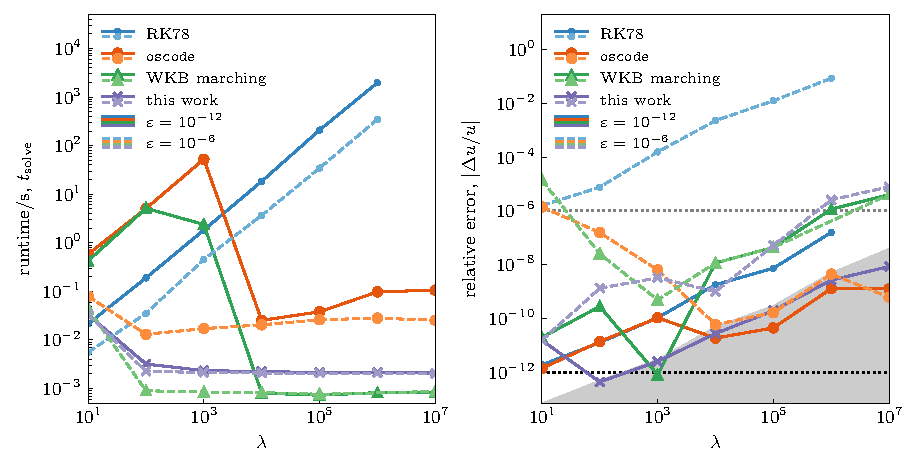
\includegraphics{plots/bremer237-timing.pdf}
    \caption{\label{bremer237-timing} Performance comparison of our solver (ARDC) and
    other state-of-the-art algorithms on \cref{bremer237eq}. The left panel
    shows the total runtime of the solvers listed in \cref{solvercomp} as the
    frequency parameter $\lambda$ is varied, for two different relative
    tolerance settings: runtimes with $\varepsilon = 10^{-12}$ are plotted with
    solid, and $\varepsilon = 10^{-6}$ with dashed lines. The right panel shows
    the corresponding relative error the solvers achieved at the end of the
    integration interval. The grey shaded region in this plot serves as an
    upper bound on any errors that fall within it, since the errors plotted
    here were computed using the Kummer's phase function method as a reference, which is
    only accurate up to the upper edge of the grey region.}
\end{figure}




\subsection{Special function evaluation: Legendre's equation}
% Previously: Evaluating special function evaluation: Legendre's equation
% department of redundancy department

Being able to solve highly oscillatory ODEs accurately means the solver can
quickly evaluate high-order special functions that obey an ODE of the required
form, such as Legendre's differential equation,
\be\label{legendreode}
(1-t^2)u'' - 2tu' + n(n+1)u = 0, \quad t \in [0.1, 0.9]. 
\ee
The problem need not be phrased as an initial value problem: due to the
linearity of the ODE, two arbitrary linearly independent solutions can be
linearly combined to satisfy initial or boundary conditions. In this example,
the results of which are shown in \cref{legendre-results}, we set tolerances of
$\varepsilon = 10^{-12}$, $\varepsilon_h = 10^{-13}$ and the number of
Chebyshev nodes in oscillatory steps to $n = 16$. 
% Imprecise again, number of nodes is (n+1)
These results again demonstrate the frequency-independence of the runtime of
our algorithm and show that the required tolerance (where the condition number
of the problem allows) is achieved. Note that after the solution of the ODE has
taken place, evaluating $u$ at intermediate points (\ie not at the internal
timesteps taken by the solver) is possible via interpolation of the phase
function $x$ in $\bigO(1)$ time, independently of the order $n$ in \cref{legendreode}.


\begin{table*}
    \renewcommand{\arraystretch}{1.2}
    \resizebox{\textwidth}{!}{\begin{tabular}{l c c c c c c c c c c}
\hline \hline 
$n$  &  $\max|\Delta u/u|$  &  $t_{\mathrm{solve}}$/\si{\s}  &  $t_{\mathrm{eval}}$/\si{\s}  &  $n_{\mathrm{s,Ricc}}$  &  $n_{\mathrm{s,Cheb}}$  &  $n_{\mathrm{s,tot}}$  &  $n_{\mathrm{f}}$  &  $n_{\mathrm{LS}}$  &  $n_{\mathrm{LU}}$  &  $n_{\mathrm{sub}}$ \\ \hline
%$10^1$  &  $2.25 \times 10^{-12}$  &  $0.00814$  &  $0.0$  &  $11$  &  $2922$  &  $23$  &  $1$  &  $0$ \\ 
%$10^2$  &  $1.33 \times 10^{-10}$  &  $0.03$  &  $0.0$  &  $33$  &  $8499$  &  $59$  &  $1$  &  $19$ \\ 
%$10^3$  &  $6.67 \times 10^{-12}$  &  $0.00355$  &  $0.0$  &  $8$  &  $1028$  &  $1$  &  $1$  &  $8$ \\ 
%$10^4$  &  $9.93 \times 10^{-11}$  &  $0.00303$  &  $0.0$  &  $8$  &  $1028$  &  $1$  &  $1$  &  $8$ \\ 
%$10^5$  &  $8.72 \times 10^{-10}$  &  $0.00316$  &  $0.0$  &  $8$  &  $1028$  &  $1$  &  $1$  &  $8$ \\ 
%$10^6$  &  $7.41 \times 10^{-9}$  &  $0.00264$  &  $0.0$  &  $8$  &  $1028$  &  $1$  &  $1$  &  $8$ \\ 
%$10^7$  &  $9.99 \times 10^{-8}$  &  $0.00255$  &  $0.0$  &  $8$  &  $1028$  &  $1$  &  $1$  &  $8$ \\ 
%$10^8$  &  $6.72 \times 10^{-7}$  &  $0.00269$  &  $0.0$  &  $8$  &  $1028$  &  $1$  &  $1$  &  $8$ \\ 
%$10^9$  &  $1.17 \times 10^{-5}$  &  $0.00287$  &  $0.0$  &  $8$  &  $1028$  &  $1$  &  $1$  &  $8$ \\ 
$10^1$  &  $2.25 \times 10^{-12}$  &  $0.00995$  &  $0.0$  &  $(0, 0)$  &  $(11, 11)$  &  $(11, 11)$  &  $2922$  &  $23$  &  $1$  &  $0$\\ 
$10^2$  &  $1.33 \times 10^{-10}$  &  $0.0313$  &  $0.0$  &  $(19, 4)$  &  $(29, 29)$  &  $(48, 33)$  &  $8499$  &  $59$  &  $1$  &  $19$\\ 
$10^3$  &  $6.67 \times 10^{-12}$  &  $0.0035$  &  $0.0$  &  $(8, 8)$  &  $(0, 0)$  &  $(8, 8)$  &  $1028$  &  $1$  &  $1$  &  $8$\\ 
$10^4$  &  $9.93 \times 10^{-11}$  &  $0.00329$  &  $0.0$  &  $(8, 8)$  &  $(0, 0)$  &  $(8, 8)$  &  $1028$  &  $1$  &  $1$  &  $8$\\ 
$10^5$  &  $8.72 \times 10^{-10}$  &  $0.00259$  &  $0.0$  &  $(8, 8)$  &  $(0, 0)$  &  $(8, 8)$  &  $1028$  &  $1$  &  $1$  &  $8$\\ 
$10^6$  &  $7.41 \times 10^{-9}$  &  $0.0026$  &  $0.0$  &  $(8, 8)$  &  $(0, 0)$  &  $(8, 8)$  &  $1028$  &  $1$  &  $1$  &  $8$\\ 
$10^7$  &  $9.99 \times 10^{-8}$  &  $0.00314$  &  $0.0$  &  $(8, 8)$  &  $(0, 0)$  &  $(8, 8)$  &  $1028$  &  $1$  &  $1$  &  $8$\\ 
$10^8$  &  $6.72 \times 10^{-7}$  &  $0.00312$  &  $0.0$  &  $(8, 8)$  &  $(0, 0)$  &  $(8, 8)$  &  $1028$  &  $1$  &  $1$  &  $8$\\ 
$10^9$  &  $1.17 \times 10^{-5}$  &  $0.0024$  &  $0.0$  &  $(8, 8)$  &  $(0, 0)$  &  $(8, 8)$  &  $1028$  &  $1$  &  $1$  &  $8$\\ 
\hline \hline
\end{tabular}
}
    \caption{Accuracy, runtime and evaluation statistics of the present algorithm when
    applied to Legendre's differential equation, \cref{legendreode}. The column
    headers are identical to those in \cref{bremer237tab} and are explained in
    the text. \label{legendre-results}}
\end{table*}


%\subsection{An example from cosmology \label{cosmo-example-sec}}
%
%%One might be tempted to think that considering the damping-free form ($\g(t) =
%%0$) of \cref{ode} would have been sufficient, and that allowing for the case of
%%$\g(t) \neq 0$ does not add generality, since the $\g$-term in \cref{ode} may
%%always be removed via a variable transform. Indeed, it can be shown that either
%%the independent or the dependent variable can be rescaled to yield a
%%damping-free ODE. The most general transformation that preserves the linearity
%%of the ODE is
%%\be\label{transformation}
%%t \to \tau := f(t), \quad u \to y:= g(\tau)u,
%%\ee
%%which yields the second-order linear ODE
%%\be\label{transformed-ode}
%%\ddot{y} + \left[ \frac{2\dot{g}}{g} + \frac{f''}{(f')^2} + \frac{2\g}{f'} \right]\dot{y} + 
%%\left[\ddot{g} + \left( \frac{f''}{(f')^2} + \frac{2\g}{f'} \right)\frac{\dot{g}}{g} + \frac{\om^2}{(f')^2} \right]y = 0,
%%\ee
%%where the overdot denotes differentiation with respect to $\tau$. Setting the coefficient of $\dot{y}$ to zero yields the constraint
%%\be
%%2\tilde{\g} = \frac{2\dot{g}}{g} + \frac{f''}{(f')^2} + \frac{2\g}{f'} = 0,
%%\ee
%%and simplifies the frequency of the transformed ODE to
%%\be
%%\tilde{\omega}^2 = \ddot{g} - 2\left( \frac{\dot{g}}{g}\right)^2 + \left( \frac{\om}{f'}\right)^2.
%%\ee
%%This, however, still carries a functional degree of freedom, in that one is free to choose $g$ (or $f$). Despite the fact that the ODE may always be transformed this way, in some cases it is not numerically stable to do so. We demonstrate this through an example taken from cosmology.
%
%A widely accepted theory explaining the origin of large-scale structure in the Universe is that of inflation \cite{baumann2022}. Preceding and during an early phase of exponential expansion, quantum-scale fluctuations in matter density (and hence spacetime-curvature) evolved according to the Mukhanov--Sasaki equation,
%\be\label{mseq}
%\frac{\d^2 \mathcal{R}_k}{\d N^2} + 2\g(N)\frac{\d \mathcal{R}_k }{\d N} + \om^2(N) \mathcal{R}_k = 0, 
%\ee
%where the independent variable is the number of e-folds of inflation, $N = \ln
%a$, with $a$ being the scale factor, a time-dependent characteristic
%lengthscale associated with the expansion. During inflation, $a$ grows
%exponentially, making $N$ a natural independent variable for the purposes of
%computation. $\mathcal{R}$ is a time-dependent scalar field that quantifies
%perturbations in the spatial curvature of spacetime called the gauge-invariant
%curvature perturbation. $\mathcal{R}_k$ is then the Fourier component of
%$\mathcal{R}$ associated with the wavenumber $k$. The damping term and
%frequency in \cref{mseq} are time- ($N$-) and wavenumber ($k$-) dependent, as
%well as functions of the underlying cosmological model. An example
%for their behaviour is shown in the top left panel of \cref{cosmology-example}.
%The bottom left panel then shows the evolution of a single perturbation mode
%$\mathcal{R}_k$ corresponding to a lengthscale of\footnote{When the perturbation mode is governed by
%the Mukhanov--Sasaki equation, the Universe is in its primordial phase of
%inflation, approximately $10^{-32}$ \si{\s} after the Big Bang. These primordial
%perturbations later translate into anisotropies in the temperature and
%polarisation of the Cosmic Microwave Background (CMB), which we can observe
%today. The CMB anisotropies are observed over the celestial sphere and are thus broken
%down into spherical harmonics parametrised by their multipole moment
%$\ell$. Even though a single plane wave projected onto a sphere generates
%anisotropies on multiple scales, the dominant anisotropy it generates will have
%$\ell \approx kD_{\ast}$ \cite{hu1995}, where $D_{\ast}$ is the angular
%diameter distance to the surface of last scattering, measured in
%\si{\mega\parsec}. The scale we consider in the text corresponds to the
%resolution of the current CMB experiments, \ie the largest currently observable
%multipole, $\ell \approx 2000$, or a wavenumber of \SI{0.2}{\per\mega\parsec}.
%} \SI{0.2}{\per\mega\parsec}. The perturbation mode exhibits rapid oscillations
%before it ``freezes out'' at a constant amplitude at which it will remain until
%after the end of primordial inflation. In cosmology, it is this frozen-out
%amplitude we are interested in computing, so the perturbation modes are evolved numerically
%until well into the constant-amplitude regime. Towards the end of the
%integration regime $\om \approx 0$ and $\g \approx \text{const.}$, giving the
%solution
%\be\label{infl-sol-1}
%\mathcal{R}_k \approx C_0 - \frac{C_1}{\g}e^{-\g N},
%\ee
%which quickly converges to $\mathcal{R}_k \approx C_0$. Once this phase of the
%numerical solution is reached, the condition number of the problem does not increase
%significantly -- intuitively, it is the constant part of the solution that is
%of interest, which is easy to follow numerically. Transforming the
%dependent variable to yield the damping-free equation of motion 
%\be
%\frac{\d^2 \tilde{\mathcal{R}}_k}{\d N^2} + \tilde{\om}^2(N) \tilde{\mathcal{R}}_k = 0, 
%\ee
%with $\tilde{\om}^2 = \om^2 + \g' - \g^2$, results in the behaviour plotted on
%the left-hand-side of \cref{cosmology-example}. In the region where the
%perturbation mode's amplitude was previously constant we now have $\tilde{\om}
%< 0$ and $\tilde{\om} \approx \text{const.}$, giving 
%\be
%\tilde{\mathcal{R}}_k \approx C_2 e^{+\tilde{\om}N} + C_3 e^{-\tilde{\om}N}.
%\ee
%The physically meaningful solution is the exponentially
%growing one. It is possible to follow this solution closely, but in this
%formulation the condition number of the problem grows proportionally with
%$|\tilde{\om}N|$, regardless of whether the solution
%is oscillatory or exponential, costing valuable digits.
%
%The primordial power spectrum (PPS) of curvature perturbations is defined as the function
%\be
%\mathcal{P}_{\mathcal{R}}(k) = \frac{k^3}{2\pi^2} |\mathcal{R}_k|^2,
%\ee
%where $|\mathcal{R}_k|$ is taken as the frozen-out amplitude of the given perturbation mode. 
%In cosmological inference, forward modelling often starts from the PPS which is
%computed assuming some set of cosmological parameters. For each PPS
%computation, one needs to solve \cref{mseq} for $\mathcal{O}(10^3)$ values of
%$k$, and around $\mathcal{O}(10^7 - 10^9)$ likelihood evaluations (each of
%which involves one PPS calculation) are necessary for mapping the posterior
%probability distribution. This gives a total of {$\mathcal{O}(10^{10} -
%10^{12})$} numerical solves of the highly oscillatory \cref{mseq}, which is only
%feasible if an extremely efficient, specialised numerical method is used. Moreover, the above reasoning demonstrates that the numerical method needs to be able to deal with a non-zero $\g$-term.   
%
%\begin{figure}[tbp]
%    \centering
%    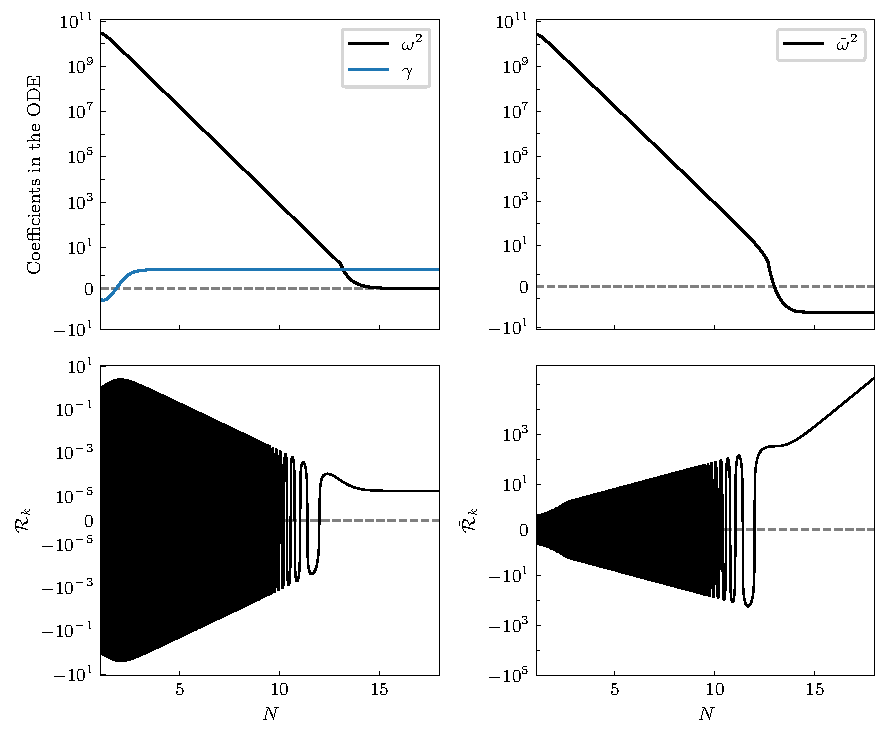
\includegraphics{plots/cosmology.pdf}
%    \caption{\label{cosmology-example} Plot illustrating the change in the
%    terms in the Mukhanov--Sasaki equation \cref{mseq} and the behaviour of its
%    solution upon transforming to $\gamma$-free form. The top panels show the
%    frequency and damping term (where applicable) in the ODE as a function of
%    the e-folds of inflation $N$, while the bottom panels shows the evolution
%    of the dependent variable, the gauge-invariant curvature perturbation
%    $\mathcal{R}_k$ of comoving wavenumber $k$ corresponding to an 
%    observable lengthscale of \SI{0.2}{\per\mega\parsec}. Note the
%    symmetric-logarithmic scales on all $y$-axes, which is linear close to
%    zero but logarithmic otherwise. }
%\end{figure}


\section{Conclusions \label{conclusions}}

% Summary of paper
We presented an efficient numerical algorithm for solving linear second order
ODEs of a single variable, posed as initial value problems (see \cref{ode}), whose solution
might be highly oscillatory for some regions of the solution interval.
The
algorithm's runtime is independent of the characteristic frequency of
oscillations, like that of a few contemporary solvers that exploit asymptotics to speed up computation in the highly oscillatory region.
Our solver is an improvement on these contemporary solvers
in three ways: it is capable of solving the ODE efficiently regardless of
whether its solution oscillates or not; it is arbitrarily high-order accurate;
and it solves a more general problem by not imposing the restriction $\gamma =
0$ in \cref{ode}. 
We described the two methods making up the algorithm which works by
time-stepping, the mechanism by which the stepsize is adapted based on local
error estimates, and the procedure that decides which of the two methods to
use. One of the methods is a spectral solver based on Chebyshev nodes, while
the other is a numerical functional iteration that generates an asymptotic
solution for the Riccati form of the ODE. This amounts to constructing a
non-oscillatory phase function (logarithm of the dependent
variable). The error in this asymptotic expansion was measured in terms of the
residual of the Riccati equation. We have shown that given a sufficiently
slowly varying and large $\om$ and suficiently small $\g$, this residual
converges geometrically for the first $k$ iterations, but at a rate that
deteriorates with $k$. We formalised and proved this statement in \cref{TR},
and illustrated this temporary convergence in a numerical experiment. Further
numerical experiments confirmed the convergence of the overall algorithm and
compared its performance with that of state-of-the-art and standard solvers.

% Future work
% Allow for imaginary $\om$
Within the scope of this work, we only allowed $\om^2 \geq 0$. When $\om$ is
imaginary, any standard numerical solver will pick up the exponentially growing
solution due to rounding error, which will quickly overpower the evanescent
solution. A similar asymptotic approach, however, is possible as in the
oscillatory case, in that one can construct two series solutions to the Riccati
equation which form a complete basis for \cref{ode} and can thus be linearly
combined and the desired (evanescent or growing) solution can be selected for
each timestep. Care needs to be taken in regions where $|\om|$ is not large
enough for the asymptotic expansion to be sufficiently accurate.

% BVPs
Although we focused on initial value problems, note that due to the linearity
of the ODE any set of auxiliary conditions can be satisfied as a
post-processing step by solving the ODE with two sets of linearly indipentend
initial conditions and linearly combining the resulting solutions.

% Error analysis
It is left to a future analysis to relate the residual of the Riccati equation
\cref{ricc} or the original ODE \cref{ode} to an estimate of the solution's
local error. This would make the error control more uniform across the
different types of steps our algorithm uses and is the quantity being
controlled in typical numerical solvers.  

% Global spectral method ~ Chebop
Spectral methods are usually applied over the entire solution interval (\eg in
\cite{driscoll2008}) rather than within a time-stepping framework. When applied
locally and over a stepsize that can be changed adaptively, a degeneracy
appears between the number of nodes $n$ and the stepsize $h$, in that $n$ can
be increased and $h$ can be decreased to lower the local error. This degeneracy
could potentially be broken by determining the points at which the algorithm is
supposed to switch between Riccati and Chebyshev steps \emph{a priori}, or at
least identifying large regions of the solution interval where the Chebyshev
spectral will need to be used, and solving the ODE in these regions with a
single application of the spectral method with large $n$. Using \eg a sparse
spectral element method \cite{fortunato2021}, the solution of these regions
could be made more efficient.

% Quadrature
The piecewise-continuous numerical solution $\tilde{u}(t)$ our algorithm generates is made up
of sections represented by polynomials or exponentials of polynomials with
complex coefficients. Both of these are analytic in the complex plane, and so
it may be possible to calculate $\int_a^b \tilde{u}(t)\mathrm{d}t$ quickly,
despite $\tilde{u}$ being highly oscillatory for some or all of $[a, b]$, by
finding an appropriate contour in the complex plane. The more oscillatory
$\tilde{u}$, the faster it decays along the imaginary axis, and so the smaller
the number of quadrature points required to compute the numerical integral to a
given accuracy. This application will be explored in a future paper.
% PDEs???

*** TO INSERT: analysis question is to prove the discretized
defect correction matches the continuous, ie, bound discretization error.
And study the discrete iteration.


\section*{Acknowledgments}
We have benefitted greatly from discussions with Jim Bremer, Charlie Epstein,
Manas Rachh, and Leslie Greengard.
The Flatiron Institute is a division of the Simons Foundation.


%%%%%% suggest move this to comments.txt:

% Some things left to do:  (are this FA or AB ones? Are some obsolete?) These are for FA! Some may be obsolete.
% AB comments with "-"

% Figure for complex plane setup for proof of thm 3
% - sure, get from your talk.

% Numerically stable residual iterations!
% - not sure what you mean

% Final description of stepsize algorithm 
% Flowchart?
%  - imprt from talk

% Cosmo stuff? (Paper is too long!)
% - see once finer edit.

% Bremer's basic iteration (worked it out on paper but paper is already too long)
% - add footnote saying other iterations exist, give Bremer's. Note it
% needs sqrt which bring branch issue.

% Some comment that although theorem is pointwise convergence, uniform convergence over some interval is trivial by enclosing it in a larger ball.}
%  - ok, put in Sec 3.

% Relate the ball in the theorem to the interval size that can be well-approximated by $p$th order Cheby, using Bernstein ellipse of Tref
% - too much for here.

% From [residual of ODE and Riccati] to solution error bounds, maybe? This is similar to local discretization err in a more typical numerical solver. (check LeVeque, Tref, Hairer, etc).
% - too hard, state in Discussion.

% Numerical results to support deterioration of convergence rate r with total iteration number k in Thm (figure?)
% - no you have this in Fig 1 right?

% More references needed
% - just in intro


\begin{comment}    % we don't want to see this int he paper...
\Fruzsi{
\section{List of changes}

\begin{itemize}
    \item{General
        \begin{itemize}
            \item{Formatted cref so that equations appear in brackets without the ``Eq.'' in front.}
            \item{Removed $t_{\mathrm{eval}}$ from tables and text since not measured.}
            \item{Added a two-panel figure showing 1) a flowchart of the algorithm and 2) the complex plane setup for the proof of the convergence of Riccati iteration.}
            \item{Our method has a name now! \texttt{cascade}: \textbf{c}ode for \textbf{a}daptive \textbf{s}pectral Ric\textbf{ca}ti \textbf{d}efect corr\textbf{e}ction. Used this in the legend in \cref{bremer237-timing}. $\to$ The code will probably be a part of \texttt{oscode}, so I dropped this and are just referring to the method in the relevant figure as RDC -- Riccati defect correction. }
        \end{itemize}
    }
    \item{Abstract
        \begin{itemize}
            \item{Changed title to be shorter, ``arbitrarily high-order'' to spectral, added adaptivity.}
            \item{Scope of work sounded too narrow, so removed ``ODE of a single dependent variable'', and added BVPs.}
            \item{Reordered introduction to methods and added more detail for Riccati steps.}
            \item{Added comparison to other solvers.}
        \end{itemize}
    }
    \item{Introduction
        \begin{itemize}
            \item{Removed bit on oscillatory behaviour in ODEs arising in different ways (was thinking about oscillatory forcing terms, coupled first-order ODEs, etc).}
            \item{Added examples for ODEs of interest in areas of physics and engineering, with citations. Added argument that our method could replace analytic asymptotics applied by hand.}
            \item{Changed criteria on $\om$, $\gamma$ as per suggestion.}
            \item{Notation change $i \to j$ in WKB ansatz, also compressed to one line.}
            \item{Discussed complex ODE coefficients.}
            \item{Clarified wording in problem statement, \eg discretization nodes instead of time-points.}
            \item{Added QLM citations. Concerncs: Mandelzweig 2004 is a preprint -- physics journals usually don't like authors citing papers that haven't been peer-reviewed. }

        \end{itemize}
    }

    \item{Numerical results
        \begin{itemize}
            \item{Added Corollary after $\kappa$ definition to state maximum achievable accuracy, and referred to this from the Airy equation subsection.}
            \item{Airy equation: refined justification of this test case, addded new paragraph to point to the convergence plot (right panel of \cref{convergence-plot}).}
            \item{Going to refer to Bremer's work as phase function method rather than Kummer's phase function method, I think that would be too long.} 
            \item{Added DLMF citation to Airy functions.}
        \end{itemize}
    }
\end{itemize}

}
\end{comment}

% BBBBBBBBBBBBBBBBBBBBBBBBBBBBBBBBBBBBBBBBBBBBBBBBBBBBBBBBBBBBBBBBBBBBBBBBBBBB
\bibliographystyle{abbrv}
\bibliography{refs}
\end{document}

